\documentclass{article}

\usepackage[utf8] {inputenc}
\usepackage {graphicx}
\usepackage {MnSymbol}
\usepackage {tikz}
\usepackage {media9}
\usetikzlibrary {arrows, shapes}
\usepackage {stmaryrd}
\usepackage {colortbl}
\usepackage {caption}
\usepackage {comment}
\usepackage {pdfpages}
\usepackage {listings}
\usepackage {color}
\usepackage {booktabs}
\usepackage {soul}
\usepackage[normalem] {ulem}

\usepackage {tcolorbox}
\usepackage {lipsum}
\usepackage {pgf}
\usepackage {etex}
\usepackage {tikz, pgfplots}

\tikzstyle {every picture} +  = [remember picture]
\everymath {\displaystyle}

\usepackage[square, numbers] {natbib} % \bibliographystyle {unsrtnat}

\hypersetup {
colorlinks = true, 
linkcolor = blue, 
filecolor = magenta, 
urlcolor = cyan, 
}

\mode<presentation> {

% The Beamer class comes with a number of default slide themes
% which change the colors and layouts of slides. Below this is a list
% of all the themes, uncomment each in turn to see what they look like.

%\usetheme{default}
%\usetheme{AnnArbor}
%\usetheme{Antibes}
%\usetheme{Bergen}
%\usetheme{Berkeley}
%\usetheme{Berlin}
%\usetheme{Boadilla}
%\usetheme{CambridgeUS}
%\usetheme{Copenhagen}
%\usetheme{Darmstadt}
%\usetheme{Dresden}
%\usetheme{Frankfurt}
%\usetheme{Goettingen}
%\usetheme{Hannover}
%\usetheme{Ilmenau}
%\usetheme{JuanLesPins}
%\usetheme{Luebeck}
%\usetheme{Madrid}
\usetheme{Malmoe}
%\usetheme{Marburg}
%\usetheme{Montpellier}
%\usetheme{PaloAlto}
%\usetheme{Pittsburgh}
%\usetheme{Rochester}
%\usetheme{Singapore}
%\usetheme{Szeged}
%\usetheme{Warsaw}

% As well as themes, the Beamer class has a number of color themes
% for any slide theme. Uncomment each of these in turn to see how it
% changes the colors of your current slide theme.

%\usecolortheme{albatross}
%\usecolortheme{beaver}
%\usecolortheme{beetle}
%\usecolortheme{crane}
%\usecolortheme{dolphin}
%\usecolortheme{dove}
%\usecolortheme{fly}
%\usecolortheme{lily}
%\usecolortheme{orchid}
%\usecolortheme{rose}
%\usecolortheme{seagull}
%\usecolortheme{seahorse}
\usecolortheme{whale}
%\usecolortheme{wolverine}

%\setbeamertemplate{footline} % To remove the footer line in all slides uncomment this line
% To replace the footer line in all slides with a simple slide count uncomment this line
\setbeamertemplate{footline}[page number]
% To remove the navigation symbols from the bottom of all slides uncomment this line
\setbeamertemplate{navigation symbols}{}
\usefonttheme {professionalfonts}
\useoutertheme {infolines}
\useinnertheme {circles}
}


\newtheorem *  {bem} {Bemerkung}

\usepackage {tikz}

\usepackage {listings}
\usepackage {color}

\definecolor {dkgreen} {rgb} {0, 0.6, 0}
\definecolor {gray} {rgb} {0.5, 0.5, 0.5}
\definecolor {mauve} {rgb} {0.58, 0, 0.82}

\lstset {frame = tb, 
language = Java, 
aboveskip = 2mm, 
belowskip = 12mm, 
showstringspaces = false, 
columns = flexible, 
basicstyle =  {\small\ttfamily}, 
numbers = none, 
numberstyle = \tiny\color {gray}, 
keywordstyle = \color {blue}, 
commentstyle = \color {dkgreen}, 
stringstyle = \color {mauve}, 
breaklines = true, 
breakatwhitespace = true, 
tabsize = 2
} % Include the file specifying the document structure and custom commands
\title{Flash Attention}
% \author{Ying Cao}
% \date{\today}

\begin{document}
\bibliographystyle{plain}

\maketitle % Print the title
\tableofcontents

\clearpage
\noindent
\linespread{1.2}
\selectfont
\setlength{\topskip}{0ex}
\setlength{\parskip}{1ex}
\setlength{\lineskip}{1em}

%---------------------------------------------------------------
% unnumbered section
%---------------------------------------------------------------

\noindent $::$ is read as "have a type of".

\noindent $\rightarrow$ is read as "maps to".

\section{Background: The Computational Process of Reduce and Map}\label{sec1}
\section[Background]{Background}

\begin{frame}[fragile]{The Transformer Architecture}

\begin{tabular}{cl}
    \begin{tabular}{c}
        \begin{tabular}{p{0.3\textwidth}p{\textwidth}}
            \scriptsize{
                The Transformer block\footfullcite{DBLP:conf/nips/VaswaniSPUJGKP17}.
            } \\
            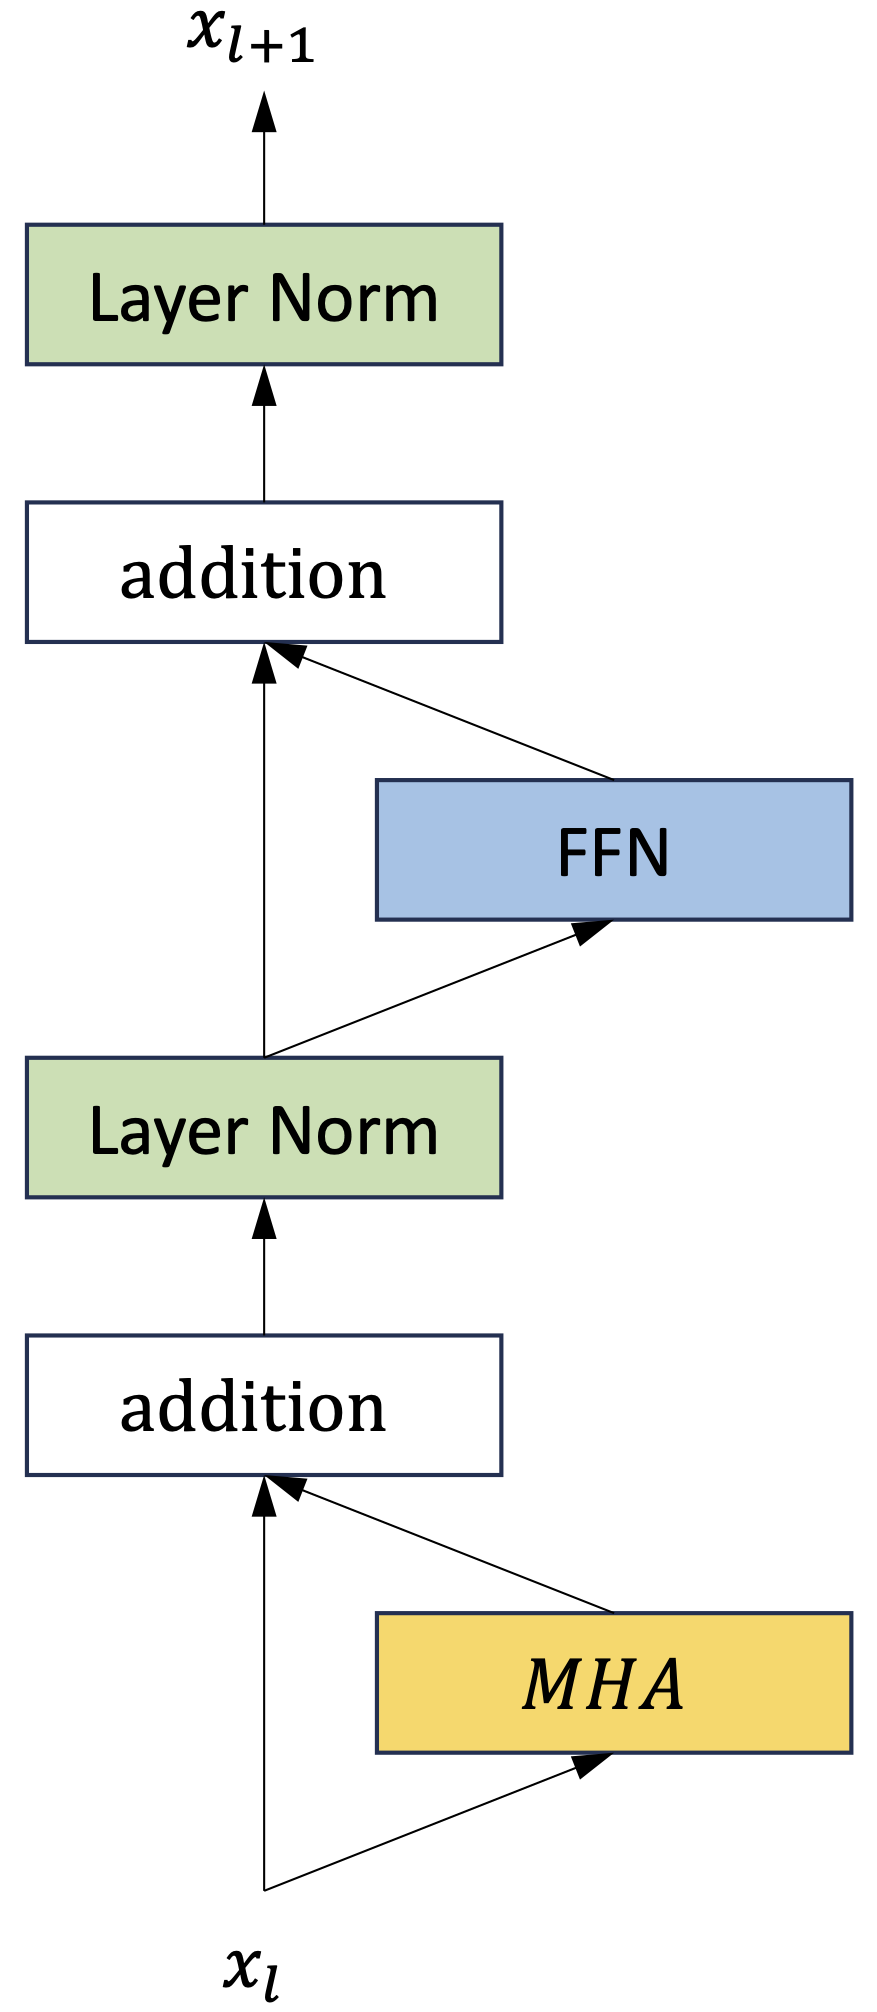
\includegraphics[scale=0.4]{"../Formalize_Flash_Attention/figures/Transformer-block.pdf"}
        \end{tabular}
    \end{tabular} &
    \begin{tabular}{p{13.5cm}l}
        \parbox{0.5 \linewidth}{
            \begin{itemize}
                \item The transformer model consists of $n_{\text{layers}}$ blocks that are stacked on top of each other.
                \item Learnable parameters in a Transformer block:
                \item[] 
                \scriptsize{
                \begin{tabular}{lll}\hline
                    \textbf{Components}& \textbf{Parameters} & \textbf{Shape} \\ \toprule[1.5pt]
                    MHA & $W_Q^i$,$W_K^i$,$W_V^i$,$W_O^i$ & $[d, d]$ \\
                    MHA & $b_Q^i$,$b_K^i$,$b_V^i$,$b_O^i$ & $[1, d]$ \\
                    layer norm & $\gamma$, $\beta$ & $[1, d]$ \\
                    FFN & $W_1^i$ & $[d, 4d]$ \\
                    FFN & $b_1^i$ & $[1, 4d]$ \\
                    FFN & $W_2^i$ & $[4d, d]$ \\
                    FFN & $b_2^i$ & $[1, d]$ \\ \hline
                    \text{In Total}&& \textcolor{red}{$12d^2+13d$}\\\hline
                \end{tabular}
                }
            \end{itemize}
        }
    \end{tabular}
\end{tabular}
\end{frame}

\begin{frame}{Estimating Storage Requirements for LLM Weights}
    \textbf{LLMs are too large to fit in the memory of a single GPU device.} Inference performance for large Transformer models can be limited by memory capacity.
    
    \begin{itemize}
        \item Storage required for LLM weights:
        \item[]
        \scriptsize{
            \begin{tabular}{lcccccc}
            \textbf{Model} & $\#\textbf{parameters}$\footnote{$\#\textbf{paramters}$ = $n_{\text{layers}}*(12d^2+13d)$. The parameters are counted in a manner that excludes word embedding and the last softmax parameters used to predict the following word.} & $n_{\text{layers}}$ & $d$ & $n_{\text{heads}}$ & $d_{\text{head}}$& $\#\textbf{storage}(GB)$\footnote{$\#\textbf{storage}$ is counted for single precision floating point number = $\#\textbf{parameters}$ * 4 / 1024 / 1024 / 1024 }\\\toprule[1.5pt]
            $\text{BERT}_{\text{base}}$ &84.94 M&12 &768 &12&64&0.3164\\
            $\text{BERT}_{\text{large}}$ &302.00 M&24 &1024 &16&64&1.1250\\
            GPT-3 small &84.94 M&12&768&12&64&0.3164\\
            GPT-3 medium &302.00 M&24&1024&16&64&1.1250 \\
            GPT-3 large &679.50 M&24&1536&16&96&2.5313\\
            GPT-3 13B &12.68 B&40&5140&40&128&47.2421 \\
            GPT-3 175B &173.95 B&96&12288&96&128&648.0006\\
        \end{tabular}
        }
        \normalsize{
        \item Other storage: Activations, \hl{K-V cache}!
        }
    \end{itemize}
    \end{frame}

\begin{frame}{LLM inference}
\footnotesize{
    \begin{itemize}
        \item[] \center{\hl{Prefill Stage}: prompts processing has large parallelism}
            \begin{enumerate}
                \item cache K-V for prompts
                    \begin{align*}
                        \mathbf{x}_K^i &= \mathbf{x}^i \cdot W_{K}^i \\
                        \mathbf{x}_V^i &= \mathbf{x}^i \cdot W_{V}^i
                    \end{align*}
                \item predict next token
                \begin{align*}
                    \mathbf{x}_Q^i &= \mathbf{x}^i \cdot W_{Q}^i \\
                    \mathbf{x}_O^i &= \textcolor{red}{\text{layernorm}}\left(\textcolor{red}{\text{softmax}}\left(\frac{\mathbf{x}_Q^i(\mathbf{x}_K^i)^T}{\sqrt{d}}\right) \mathbf{x}_V^i W_O^i + \mathbf{x}^i\right) \\
                    \mathbf{x}^{i+1} &= \textcolor{red}{\text{layernorm}}\left(\text{relu}\left(\mathbf{x}^i_OW_1^i\right)W_2^1+\mathbf{x}_O^i\right)
                \end{align*}
            \end{enumerate}
        \item[] \center{\hl{Decode Stage}: next token generation has insufficient parallelism}
            \begin{enumerate}
                \item update K-V for prompts
                        \begin{align*}
                            \mathbf{x}_K^i&\leftarrow\textcolor{red}{\text{concat}}({\mathbf{x}_K^i}, \mathbf{t}^i\cdot W_K^i) \\
                            \mathbf{x}_V^i&\leftarrow\textcolor{red}{\text{concat}}({\mathbf{x}_V^i}, \mathbf{t}^i\cdot W_V^i) 
                        \end{align*}
                \item predict next token, the same as above, but each time a token
            \end{enumerate}
    \end{itemize}
}
\end{frame}

\begin{frame}{Two stages in LLM inference}
    \begin{figure}
        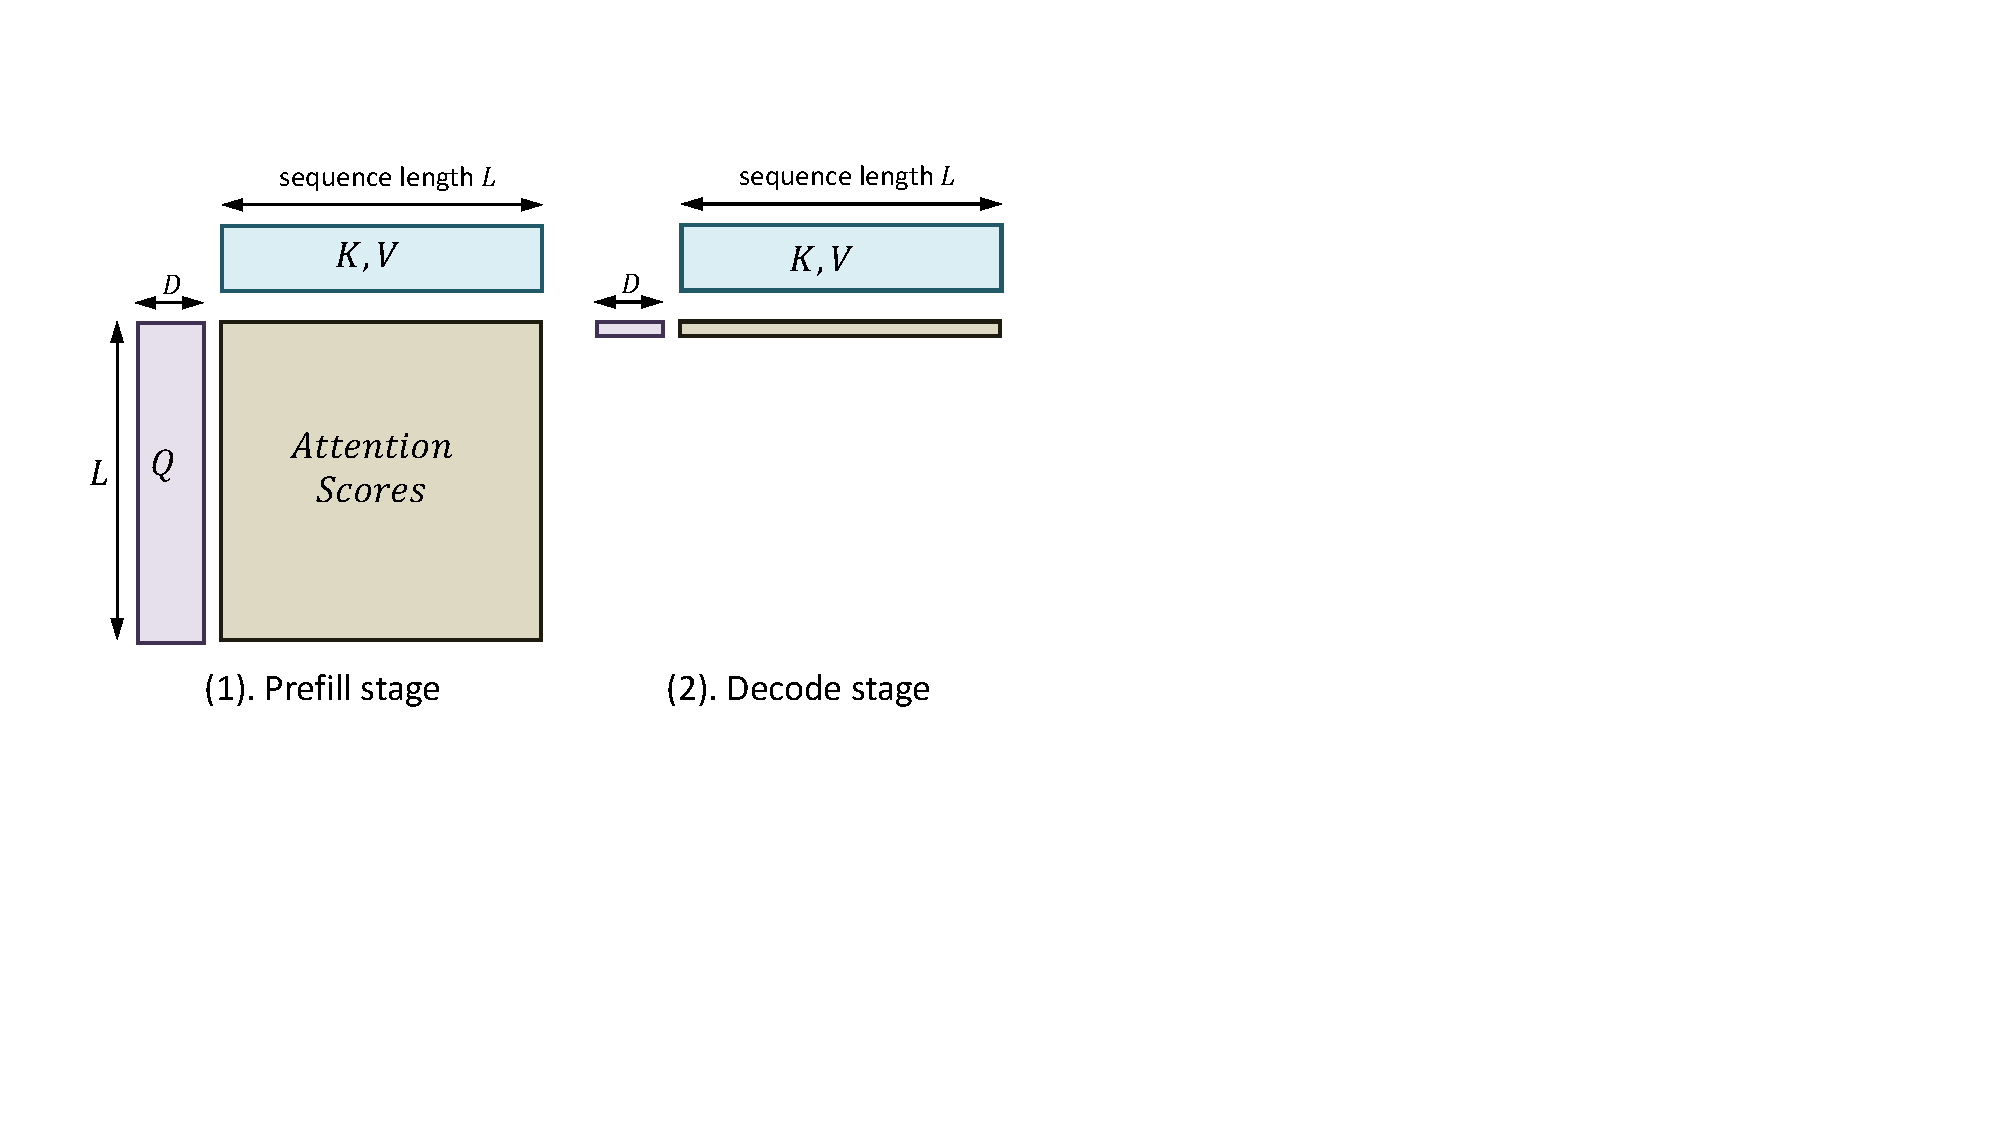
\includegraphics[width=0.7\linewidth]{./images/two-stages-in-llm-inference.pdf}
        \caption{There is a significant change in batch size between the two stages of LLM inference.}
    \end{figure}
\end{frame}

\begin{frame}{Performance Breakdown of a Transformer Block}
    \begin{figure}
        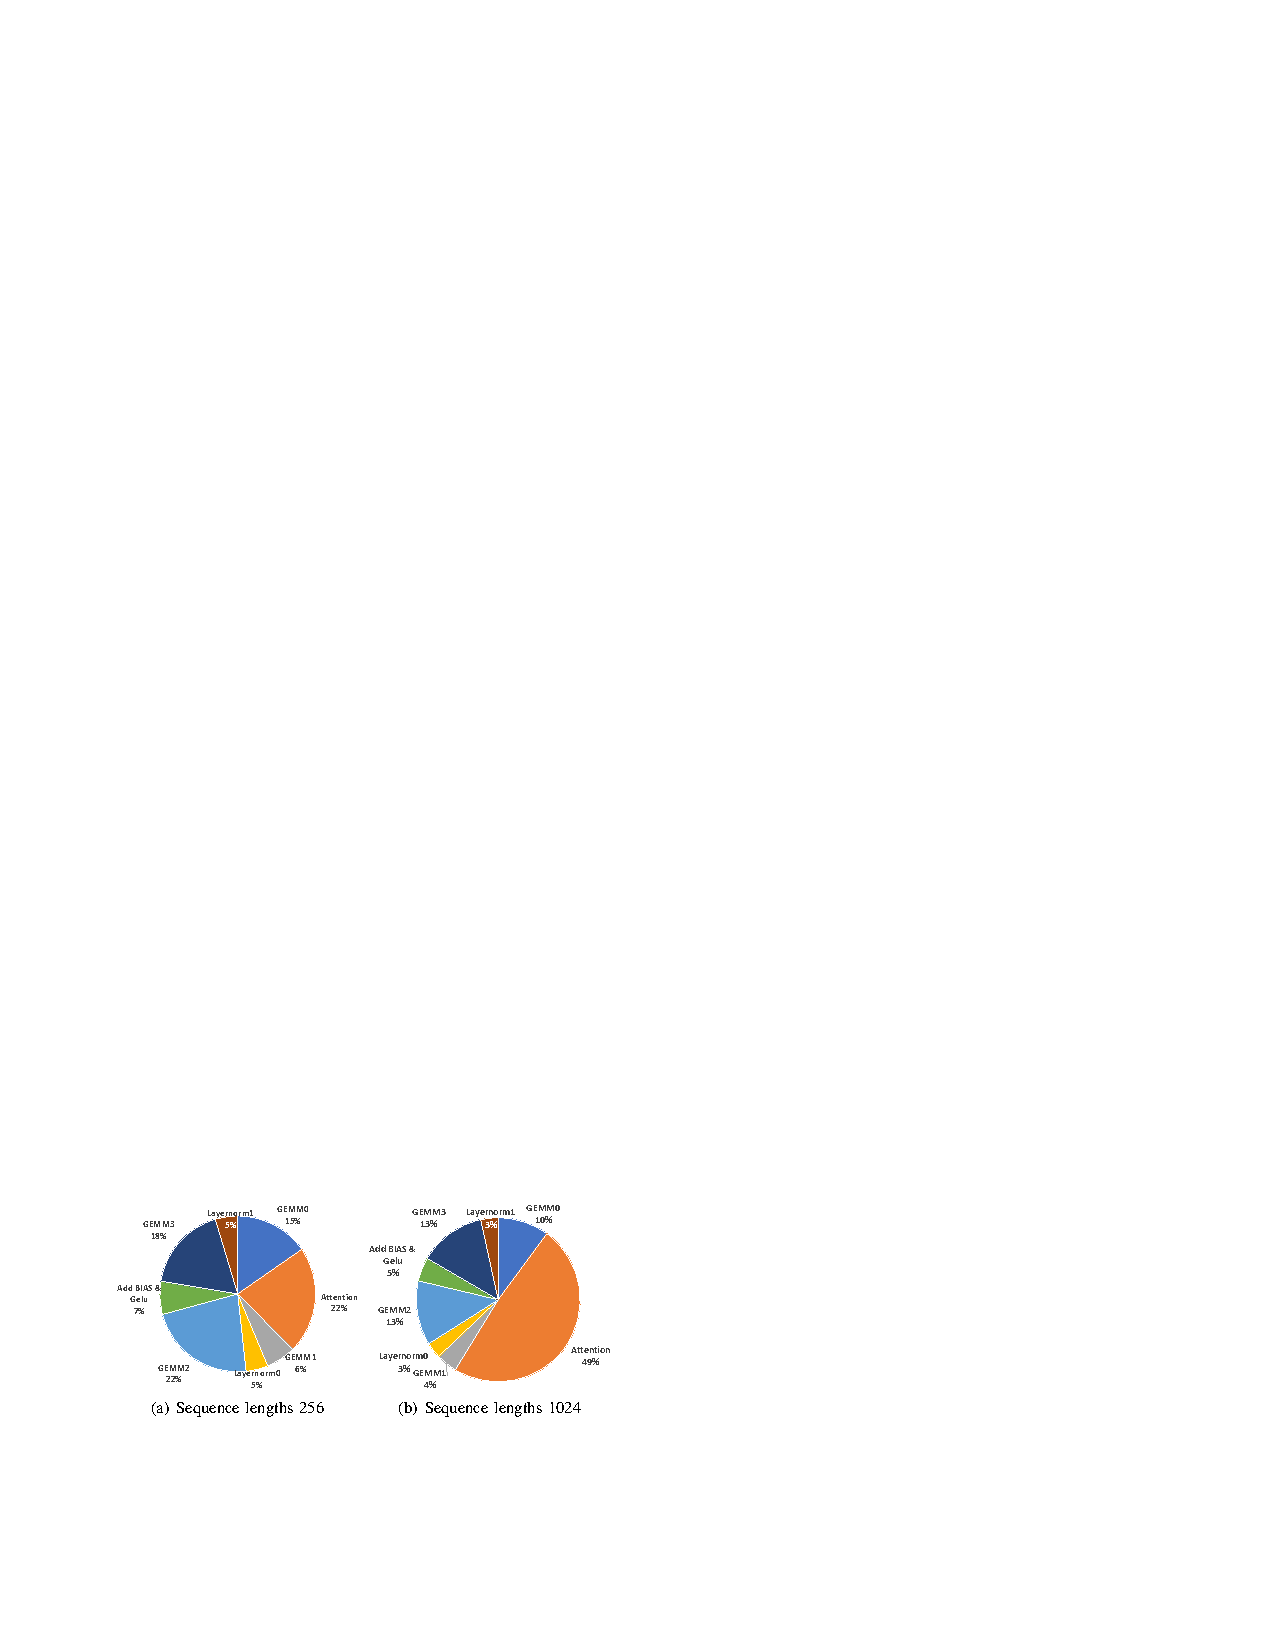
\includegraphics[width=0.7\linewidth]{./images/BERT-performance-breakdown.pdf}
        \caption{A performance breakdown of a single Transformer block\footfullcite{DBLP:journals/corr/abs-2210-03052}.}
    \end{figure}

    \footnotesize{
    \begin{enumerate}
        \item Transformer block is memory bounded.
        \item The computational complexity of MHA is quadratic to sequence length.
    \end{enumerate}
    }
\end{frame}

\begin{frame}[fragile]{Distinction Between Transformer Training and Inference:}

\textbf{Small batch size}.

\begin{enumerate}
\item Kernels are not well optimized for small batch size.

The use of \hl{skinny matrix multiplication} is a result of having a small batch size, where the batch size $N$ is much smaller than the dimensionality $d$.
\begin{align*}
 \mathbf{x}_Q^i &= \mathbf{x}^{i}W_{Q}^i & [N, d] &= [N,d] \times [d, d]\\
 \mathbf{y}_1^i &= \mathbf{x}_O^{i}W_1^i & [N, 4d] &= [N,d] \times [d, 4d]\\
 \mathbf{y}_2^i &= \mathbf{y}_1^{i}W_2^i & [N, d] &= [N,4d] \times [4d, d]\\
\end{align*}
\item \hl{Insufficient of parallelism} and performance is limited by memory bandwidth in reading weights.

\end{enumerate}
\end{frame}

\begin{frame}{FlexGen, ByteTransformer, and DeepSpeed Inference}
    \scriptsize{
        \begin{tabular}{lccc}
            &\textbf{FlexGen}\footfullcite{DBLP:journals/corr/abs-2303-06865}& \textbf{ByteTransformer\footfullcite{DBLP:journals/corr/abs-2210-03052}} & \textbf{\makecell{DeepSpeed \\Inference\footfullcite{DBLP:conf/sc/AminabadiRALLZRSZRH22}}} \\ \toprule[1.5pt]
            Throughput-oriented& yes & no & no\\
            Latency-oriented& no & yes & yes\\
            SLA& not discussed & not discussed & not discussed\\\hline
            Model&OPT-175B&BERT-like&\makecell{Dense Transformer\\MoE Transformer}\\
            Optimized Kernels&not discussed &\makecell{\textcolor{red}{yes}\\\textcolor{red}{for variable length}}&\makecell{yes\\\textcolor{red}{for small batch size}}\\
            Kernel Fusion&not discussed&yes&yes\\
            Multi-GPU&\textcolor{red}{yes}&no&\textcolor{red}{yes}\\
        \end{tabular}
    }
\end{frame}

\section{A Generalized \textit{Broadcast-and-then-Aggregate} Operation}
\subsection{The \textit{broadcast-and-then-aggregate} operation}

We consider a generalized \textit{broadcast-and-then-aggregate} operation that has the following standard form:
\lstset{
  frame=lrtb,
  backgroundcolor=\color{aliceblue},
  numbers=left,
  numbersep=1em,
  xleftmargin=1em,
  linewidth=\linewidth
}
\begin{lstlisting}[language=code_example, caption={}]
function (:$\textit{BroadcastAndThenAggregate}\ (f::(\alpha \rightarrow \gamma \rightarrow \beta), c::\gamma, \oplus::(\beta\rightarrow\theta\rightarrow \theta),\ s_0::\theta,\ xs::[\alpha])$:)  
  (:$s = s_0$:)  // initialize the accumulator
  foreach((:$x$:) in (:$xs$:))
    (:$s = \oplus(s, f(x, c))$:)  // broadcast c and accumulate s
  return (:s:)
\end{lstlisting}

The \textit{broadcast-and-then-aggregate} operation is defined by the quadruple $R=<f, c, \oplus, s_0>$.
$f$ is a function of type $\alpha \rightarrow \gamma \rightarrow \beta$, $c$ is a constant value of type $\gamma$,
$\oplus$ is a binary operator of type $\beta \rightarrow \theta \rightarrow \theta$. $s$ is an accumulator of type $\theta$ that store the aggregated value, and are initialized to $s_0$.

The computational process proceeds by enumerating each input value $x$ from the input list $xs$,
broadcasting $c$ to $x$ by applying $y=f(x, c)$, and then aggregating $s$ according to $s = s \oplus y$.
It is important to note that \textit{there is no communication among the evaluations of $f(x,c)$}.

We can use the diagram below to visualize this operation.

\begin{figure}[h]
  \centering
  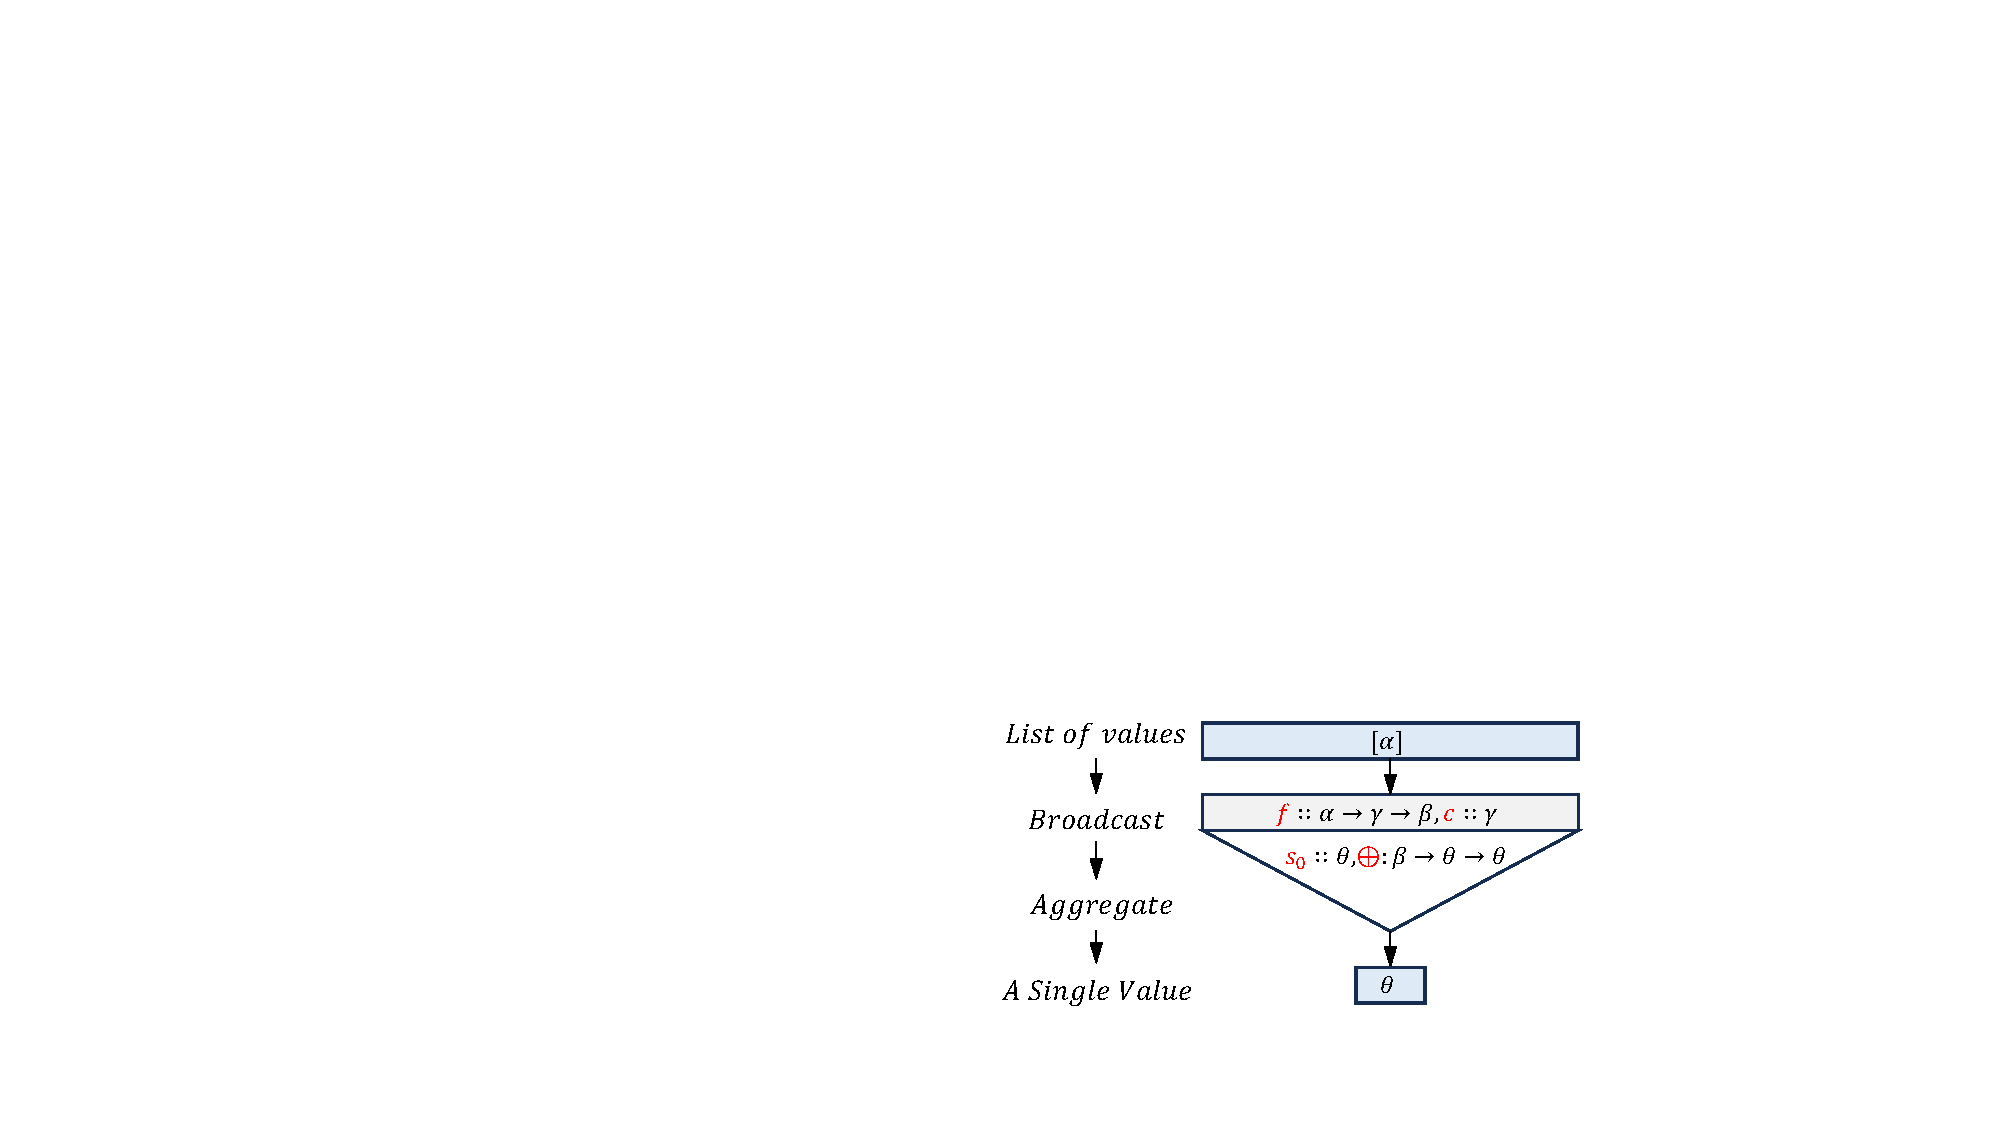
\includegraphics[width=0.4\textwidth]{figures/map_and_aggregate.pdf}
  \caption{The diagram to visualize the \textit{broadcast-and-then-aggregate} operation.}
\end{figure}

\subsection{The running example: attention in \textit{Broadcast-and-then-Aggregate}}

\textcolor{red}{Neural network computations can be expressed uniformly as a dataflow graph of broadcast-and-then-aggregate operations}.
As a concrete example, we can express attention using a set of {broadcast-and-then-aggregate} operatiosn. Figure \ref{attn} shows the corresponding dataflow graph.

\begin{equation}
\text{Attn(Q, K, V)}=\text{softmax}(QK^T)V \label{eq::attn}
\end{equation}

\begin{figure}[h]
  \centering
  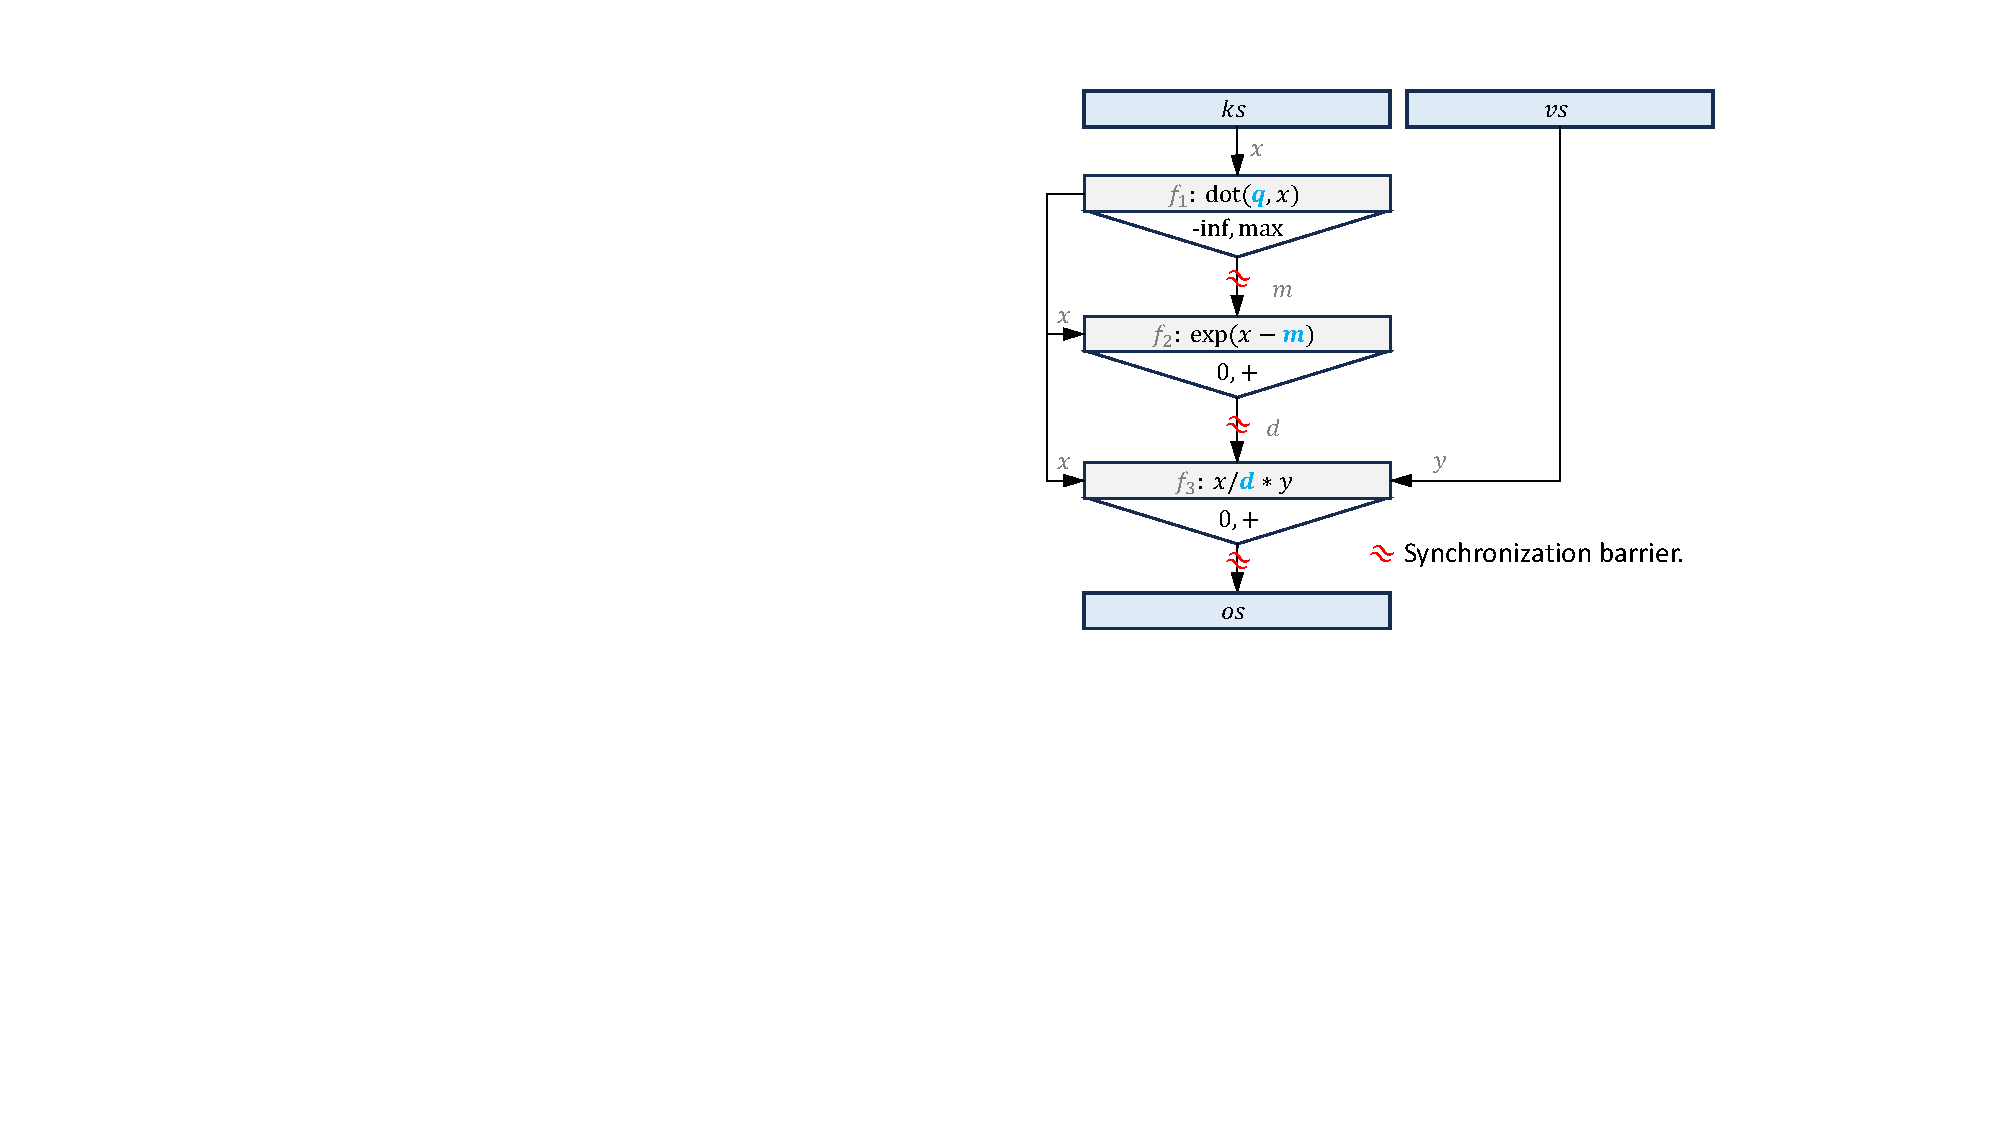
\includegraphics[width=0.5\textwidth]{figures/attention_expression_tree1.pdf}
  \caption{Express attention function using \textit{broadcast-and-then-aggregate}.}\label{attn}
\end{figure}

\section{Block Execution of a Chain of \textit{Broadcast-and-then-Aggregate}}
We use $\bar{x}=[x_1, \ldots, x_n]$ to represent a list of values, and $\bar{x}_1:\bar{x}_2$ to represent the concatenation of $\bar{x}_1$ and $\bar{x}_2$.
$f(\bar{x}) = [f(x_1, c), \ldots, f(x_n, c)]$. $s_0 \oplus \bar{x} = \textit{reduce} \ s_0\  \bar{x}$ where $s_0$ and $\oplus$ are as defined in section \ref{sec1}.

\subsection{Motivations}

\textbf{Blocked execution of a single \textit{broadcast-and-then-aggregate}}.
When the input list $\bar{x}$ is too large to be processed within hardware constraints,
We need to split it into portions that can be handled by the hardware.
By definition, the \textit{broadcast-and-then-aggregate} operation can be executed portion by portion. This means that the following equation holds:

\begin{equation}
s_0 \oplus f(\bar{x},c) = \left(s_0 \oplus f(\bar{x}_1,c)\right) \oplus \left(s_0 \oplus f(\bar{x}_2,c)\right)\ \ \ \text{where}\ \ \bar{x} = \bar{x}_1 : \bar{x}_2
\end{equation}

Assuming that the input list $\bar{x}$ is divided into two segments, $\bar{x}_1$ and $\bar{x}_2$, the broadcast stage can independently evaluate the function $f$ on each segment.
This results in $\bar{y}_1 = f(\bar{x}_1,c)$ and $\bar{y}_2 = f(\bar{x}_2,c)$, which can be executed in parallel.
The reduce operation is recursively defined and aggregates each segment independently to obtain partial aggregated results.
For example, $s_1 = s_0 \oplus \bar{y}_1$ and $s_2 = s_0 \oplus \bar{y}_2$.
These partial results are then recursively combined until a single aggregated value is obtained, such as $s = s_1 \oplus s_2$.
\textbf{\textit{If the operator $\oplus$ is both associative and commutative, the partial reduction can be computed in parallel}}.

Regarding a single \textit{broadcast-and-then-aggregate} operation, the final aggregated result depends on completing the scan of all the list inputs.
This makes the reduce operation a barrier to proceeding further.
Furthermore, if the output of the broadcast stage is required for subsequent computations,
it must be stored in memory. This requires storage proportional to the length of the input sequence.

\textbf{Motivations for blocked execution for a chain of \textit{map-and-then-aggregate} operations}.
If the input list is very long, the time it takes to scan the input and write the results of the broadcast stage (if needed) will be the dominant factor in the overall latency of the \textit{map-and-then-aggregate} operation.

If the entire computational process can be executed in parallel, with each portion computing a partial result,
an efficient implementation can exploit the memory hierarchy by caching segments of input list in high-speed memory.
Computation can then continue in high-speed memory until a synchronization barrier is met, at which point partial results must be stored in slow memory.

In the \textit{broadcast-and-then-aggregate} operation, the \textit{broadcast} stage requires storage proportional to the length of the input to store its output,
while the \textit{reduce} operation aggregates input to a smaller value that consumes less storage for its output.
If a chain of \textit{broadcast-and-then-aggregate} can proceed portion by portion in high-speed memory until the results of the broastcast stage are no longer needed by subsequent computation (and therefore do not need to be stored),
both I/O complexity and memory footprint can be reduced.

We use the attention example shown in Figure \ref{attn} as our running example. 
There are three \textit{broadcast-and-then-aggregate} operations involved.
Each can execute internally in parallel, block by block.
However, the three \textit{broadcast-and-then-aggregate} operations must execute sequentially since there are data dependences among them.
Additionally, the result of the first broadcast operation is required by the second broadcast operation, and the results of the second broadcast operation are required by the third broadcast operation.
Sequentially execute these three \textit{broadcast-and-then-aggregate} requires two storages that are proportional to the input list.

\lstset{
  frame=lrtb,
  backgroundcolor=\color{aliceblue},
  numbers=left,
  numbersep=1em,
  xleftmargin=1em,
  breaklines=true,
  linewidth=\linewidth
}
\begin{lstlisting}[language=code_example2, caption={}]
// stage1: local reducer computes partial results on individual blocks
(:$o_1$:) = Attention((:$q, ks_1, vs_1$:))     (:$o_2$:) = Attention((:$q, ks_2, vs_2$:))

// stage2: combine partial results
(:$o_{\text{new}}=\text{Combiner}(o_1,o_2)$:)
\end{lstlisting}

After the last \textit{broadcast-and-then-aggregate} operation, a noticeable decrease in storage size was observed.
Therefore, we anticipate that the entire computational process of equation (\ref{eq::attn}) be executed in two stages.
In the first stage, the input will be split into portions and partial results that require storage much smaller than the original input list will be computed without regard to original data dependencies among dependent \textit{broadcast-and-then-reduce} operations.
By selecting an appropriate block size, the entire computational process can be stored in high-speed memory.
In the second stage, a combiner will merge these partial results to obtain the correct final aggregated value.

The problems are:
\textcolor{red}{
\begin{enumerate}
    \item Under what conditions (necessary and sufficient conditions) can dependent \textit{broadcast-and-then-aggregate} operations be decomposed into these two stages?
    \item The existence of a combiner that can compute the correct final result.
    \item If such a combiner exists, how can it be constructed?
\end{enumerate}
}

\subsection{A (informal) Problem Statement}

Given two dependent \textit{broadcast-and-then-aggregate} operations:
\begin{align*}
    r &= s_0 \oplus_1 f_1(\bar{x} - c) \\
    o &= s_1 \oplus_2 f_2(\bar{y} - r)
\end{align*}

Design a combiner, denoted by $C$, that can produce an output $\Bar{\Bar{o}}$ equivalent to $o$ when computed using the following formula:
    
\begin{align*}
    r_1 &= s_0 \oplus_1 f_1(\bar{x}_1,c) && r_2 = s_0 \oplus_1 f_1(\bar{x}_2,c) \\
    o_1 &= s_1 \oplus_2 f_2(\bar{y}_1,r_1) && o_2 = s_1 \oplus_2 f_2(\bar{y}_2,r_2) \\
    \Bar{\Bar{o}} &= C(r_1, r_2, o_1, o_2)
\end{align*}

Note that a combiner $C(r_1, \bar{y}_1, r_2, \bar{y}_2)$ always exists.
This is because $r$ can be computed as $r = r_1 \oplus r_2$, and then $o$ can be re-computed using the formula $o = s_1 \oplus_2 f_2(\bar{y}_1:\bar{y}_2, r)$. 
However, implementing such a combiner would require storing the entire $\bar{y}$ and re-computing the second \textit{broadcast-and-aggregate},
which is not practical.

In order to reduce both IO complexity and the storage requirements, we must ensure that the combiners only depend on the outputs of the \textit{reduce} operations, namely $r_1$, $r_2$, $o_1$, and $o_2$.

\subsection{Preliminary Thinking to the Problem}

\textit{\textcolor{red}{Decomposable Broadcast-and-then-Aggregate Operation}}.
% A broadcast operation $F$ is decomposable under $g$ if there exists a function $h$ such that $F(x, g(c,\triangle c))=F(F(x, c), h(c,\triangle c))$.
% A decomposable broadcast $F$ under $h$ allows you broadcast the value $g(c, \triangle c)$ in two broadcast operations: first broadcast $c$ using $F$, and then broadcast an adjusting fanctor $h(c, \triangle c)$ using $F$.
We say that a \textit{broadcast-and-then-aggregate} operation $R=<F,c,s_0,\oplus>$ is decomposable under $\circ$ if there exists functions $h$ and $\odot$ such that the following equation holds:

\begin{equation}
s_0 \oplus F(\bar{x}, c \circ \triangle c)=(s_0 \oplus F(\bar{x}, c)) \odot h(c, \triangle c)\label{conds}
\end{equation}

In other words, a decomposable \textit{broadcast-and-then-aggregate} allows to broadcast a value $c \circ \triangle c$ in two steps.
First, broadcast $c$ to the input list using $F$, and then aggregate the broadcast result using $\oplus$.
Second, adjust the result of the first step with an adjusting function $h(c, \triangle c)$ using $\odot$.

% \noindent \textbf{Some examples}.

% $f(\bar{x}+c) = \bar{x} + c$ is decomposable under $+$: $f(\bar{x}+(c+\triangle c))=f(\bar{x}+c)+n\triangle c$, where $g(c, \triangle c)=n\triangle c$.
% It is also decomposable under $*$: $f(\bar{x}+c*\triangle c) = f(\bar{x~}+c) + (c * \triangle c - c)$.

% $f(\bar{x},c) = \log(c*\bar{x})$ is decomposable under $*$, but $f(\bar{x},c) = \log(c+\bar{x})$ is not decomposable under $+$.

If a \textit{broadcast-and-then-aggregate} operation can be decomposed, then a combiner $C$ exists by the definition.
Since this definitive equation(\ref{conds}) is a strict necessary condition,
and the problem is then reduced to determining the existence of the functions $\circ$ and $h$.
Unfortunately, it is easy to find counterexamples that demonstrate the non-existence of $\circ$ and $h$ for arbitrary $F$ in general case.

% \begin{align*}
%     r_1 &= s_0 \oplus_1 f_1(\bar{x}_1,c) && r_2 = s_0 \oplus_1 f_1(\bar{x}_2,c) \\
%     o_1 &= s_1 \oplus_2 f_2(\bar{y}_1,r_1) && o_2 = s_1 \oplus_2 f_2(\bar{y}_2,r_2) \\
% \end{align*}

% A correct aggregated value of the first \textit{broadcast-and-then-aggregate} can be obtained simply using: $r'= r_1 \oplus_1 r_2$.
% And the second \textit{broadcast-and-then-aggregate} should be re-computed.

% \begin{align*}
% f_1(\bar{y}_1, r') = f_1(\bar{y}_1, \textcolor{red}{h}(r_1, \triangle r_1)) = f_1(\bar{y}_1,r_1)
% \end{align*}

% Denote $\triangle r_1 := h(r', r_1)$ and $\triangle r_2 := h(r', r_2)$.
% We then re-compute the second \textit{broadcast-and-then-aggregate}:

% $f_2(\bar{y}_1, r_1 \circ \triangle r_1) = f_2(\bar{y}_1,r_1) \triangle r_1, h(r', r_1)) = f_2()$

% % \triangle r_1 &= \textcolor{red}{h}(r', r_1) && \triangle r_2 = \textcolor{red}{h}(r', r_2)\\
% % o_1 &= \\
% % \Bar{\Bar{o}} &= C(r_1, r_2, o_1, o_2)

% Given the dataflow graph Figure \ref{fused-map-and-aggreage}, let's go through flash attention step by step.
% The problem is, given partial results: $m_1$, $m_2$, $d_1$, $d_2$, $o_1$ and $o_2$, construct three combiners: $m = C_1(m_1, m_2)$, $d = C_2(m_1, m_2, d_1, d_2)$ and $o = C_3( m_1, m_2, d_1, d_2, o_1, o_2)$ to obtain an aggregated results.

% This is what flash attention does to the original attention computation.
% Figure \ref{fused-map-and-aggreage} virtualizes this process.

\begin{figure}[h]
    \centering
    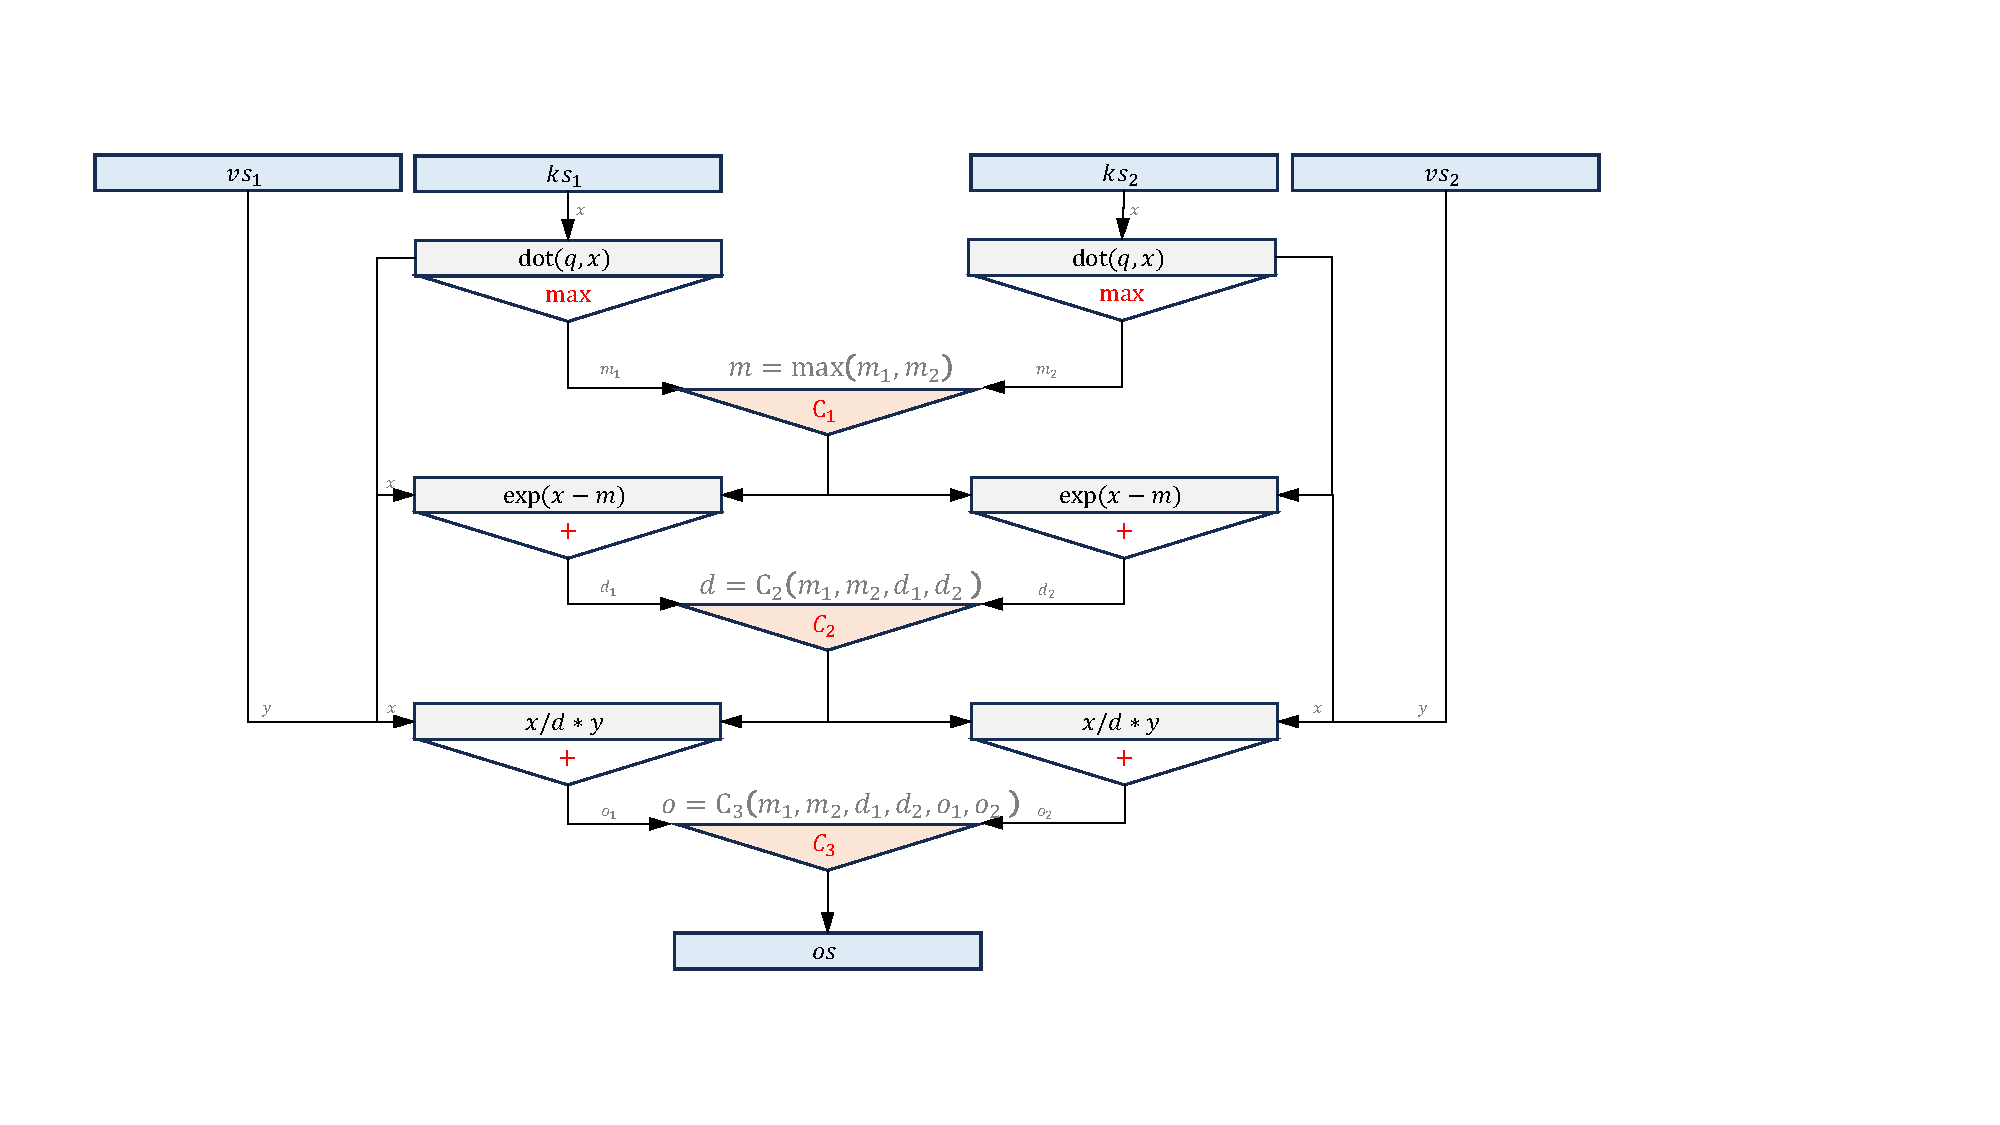
\includegraphics[width=1\textwidth]{figures/attention_expression_tree2.pdf}
    \caption{The expected blocked execution of a chain of \textit{Broadcast-and-then-aggregate}s.} \label{fused-map-and-aggreage}
\end{figure}

In the particular instance of flash attention, a combiner exists.

\colorbox{NavajoWhite}{For the first \textit{BroadcastAndThenAggregate}}, $C_1$ is trivial that is equal to the original reduce function: $m = C_1(m_1, m_2) = \max(m_1, m_2)$.

\colorbox{NavajoWhite}{For the second instance of \textit{BroadcastAndThenAggregate}}, consider the following sub-problem:
$\bar{y}_1=\exp(\bar{x}-m_1)$ has been computed for a single block,
but a new constant factor $m$ needs to be broadcast for the entire list.
This requires re-computing $\bar{y}_1' = \exp(\bar{x}-m)$.
The solution is to recover $\bar{x}$ from $\bar{y}_1$ and $m_1$ by computing: $$\bar{x}= \log(\bar{y}_1) + m_1$$

then substitue $\bar{x}$ into the equation that computes $\bar{y}_1'$. That is:

\begin{align*}
\bar{y}_1' &= \exp\left(\log \left(\bar{y}_1\right) + m_1 -m \right) \\
&= \bar{y}_1\exp(m_1 - m)
\end{align*}

Therefore:
\begin{enumerate}
\item the updating euqation for the broadcast step is: $\bar{y}_{\text{new}}=\bar{y}_{\text{old}}\exp(m_\text{old}-m_{\text{new}})$
\item combine partial results: 
\begin{align*}
   d=&C_2(d_1,d_2) = d_1 * \exp(\triangle m_1) + d_2 * \exp(\triangle m_2) \\
   \triangle m_1 :=&m_1 - \max(m_1, m_2) \\
   \triangle m_2 :=&m_2 -\max(m_1, m_2) \\
\end{align*}
\end{enumerate}

\colorbox{NavajoWhite}{For the third instance of \textit{BroadcastAndThenAggregate}}, consider the following sub-problem:
$\bar{o}_1=\frac{\bar{x}_1}{d_1}*\bar{y}$ has been computed for a single block,
but a new constant factor $d_2$ needs to be broadcast for the entire list.
This requires re-computing $\bar{o}_1' = \frac{\bar{x}_1'}{d}*\bar{y}$.
The solution is to recover $\bar{x}_1*\bar{y}$ from $\bar{o}_1$ and $d_1$ by computing: $$\bar{x}'_1 * \bar{y}= \exp(\triangle m_1)*\bar{o}_1 * d_1$$

Then the adjusted $o_1'=\frac{\exp(\triangle m_1)*o_1*d_1}{d} = o_1 *\frac{d_1 \exp({\triangle m_1})}{d_1 * \exp(\triangle m_1) + d_2 * \exp(\triangle m_2)}$, and $o = C_3(o_1, o_2) = o_1 * \frac{d_1 * \exp(\triangle m_1)}{d_1 * \exp(\triangle m_1) + d_2 * \exp(\triangle m_2)} + o_2 * \frac{d_2*\exp(\triangle m_2)}{d_1 * \exp(\triangle m_1) + d_2 * \exp(\triangle m_2)}$.


\subsection{A Counter-example: Logsoftmax instead of softmax}

\begin{figure}[h]
    \centering
    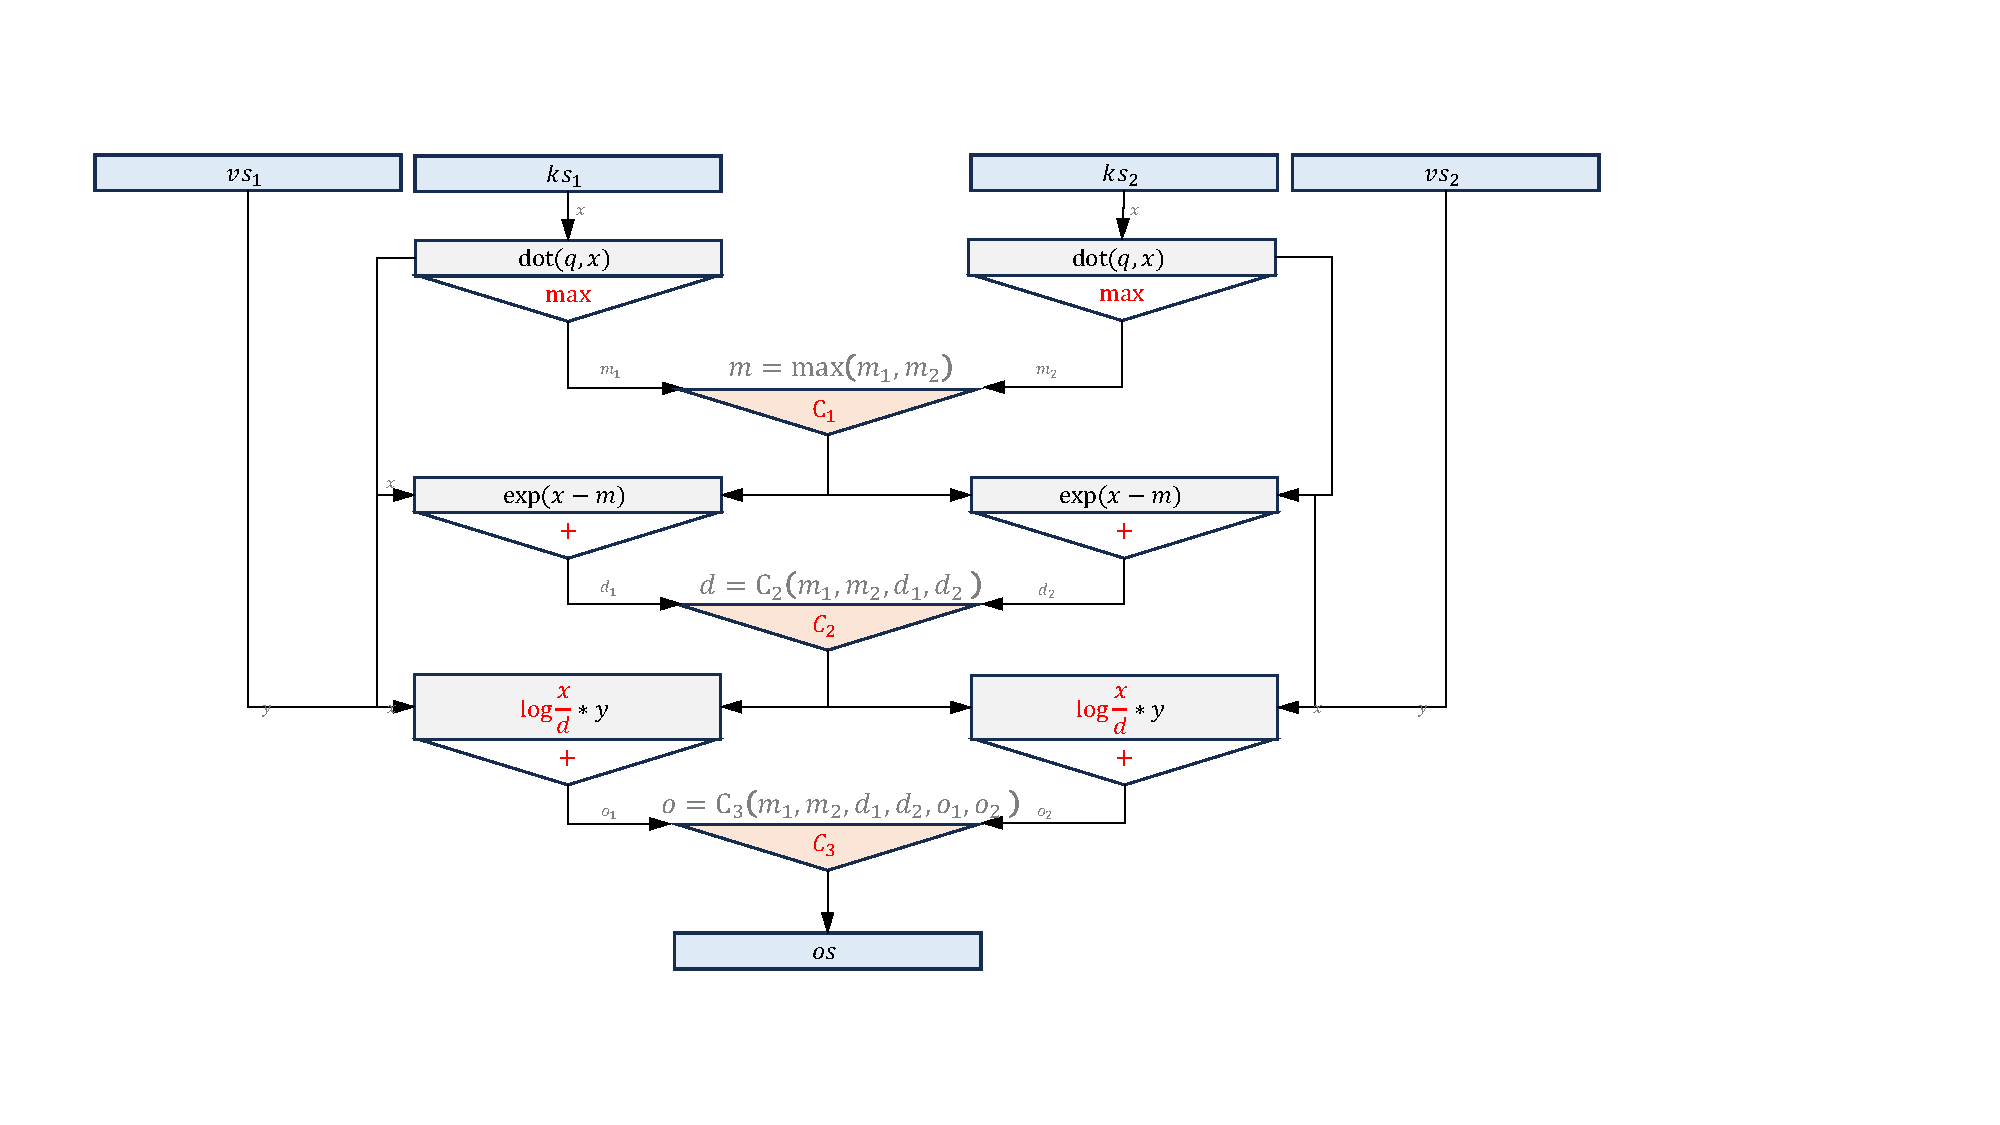
\includegraphics[width=1\textwidth]{figures/attention_expression_tree3.pdf}
    \caption{An imaginary example: use logsoftmax instead of softmax.}
\end{figure}

Let's think of an imaginary example, that compute:

$$\text{Attention}(Q, K, V) = \text{logsoftmax}(QK^T)V$$

$C_1$ and $C_2$ doest not change, thus: how $C_3$ looks like.

Suppose $\bar{z}_1$ and $o_1$ are results for the broadcast stage, and reduce stage computed on input blocks $\bar{x}_1$ and $\bar{y}$ respectively:
\begin{align*}
\bar{z}_1 &= \log\left(\frac{\bar{x}_1}{d_1}\right)*\bar{y} = \bar{y}*\log(\bar{x}_1) -\bar{y}\log d_1\\
o_1 &= \sum(0, \bar{z}_1)
\end{align*}

Then it is required to compute an updated $\bar{z}_1'$ and $o_1'$ since $\bar{x}_1$ and $d_1$ are updated.

We have:
\begin{align*}
    \bar{z}_1'&=\log \left(\frac{\bar{x}_1'}{d}\right) * \bar{y} = \bar{y}\log\bar{x}_1' - \bar{y}\log d \\
    \bar{x}_1' &= \exp(m_1 - m)\bar{x}_1 \\
    d &= \exp(m_1 -m)d_1 + \exp(m_2 -m)d_2
\end{align*}

Thus we have:
\begin{align*}
\bar{z}_1'&=\bar{y}\log\left(\exp(m_1-m)\bar{x}_1\right) - \bar{y}\log{d} \\
&=\bar{y}\left((m_1-m)+\log(\bar{x}_1)\right) -\bar{y}\log d \\
&=\bar{y}(m_1-m-\log d)+\bar{y}\log(\bar{x}) \\
&=\bar{y}(m_1-m-\log d)+\bar{z}_1+\bar{y}\log d_1 \\
&= \bar{y}(m_1-m-\log d+\log d_1)+\bar{z}_1
\end{align*}

Given $\bar{z}_1'$:
\begin{align*}
    o_1'&=\text{sum}(0, \bar{z}_1') \\
    &=(m_1-m-\log d+\log d_1)\text{sum}(0, \bar{y}) + o_1
\end{align*}

Update $o_1$ has to access its input $\bar{y}$ and compute an extra reduction sum on it.

\section{The Transformer Block}
\begin{figure}[htbp]
    \centering
    \subfigure[The Transformer block]{
        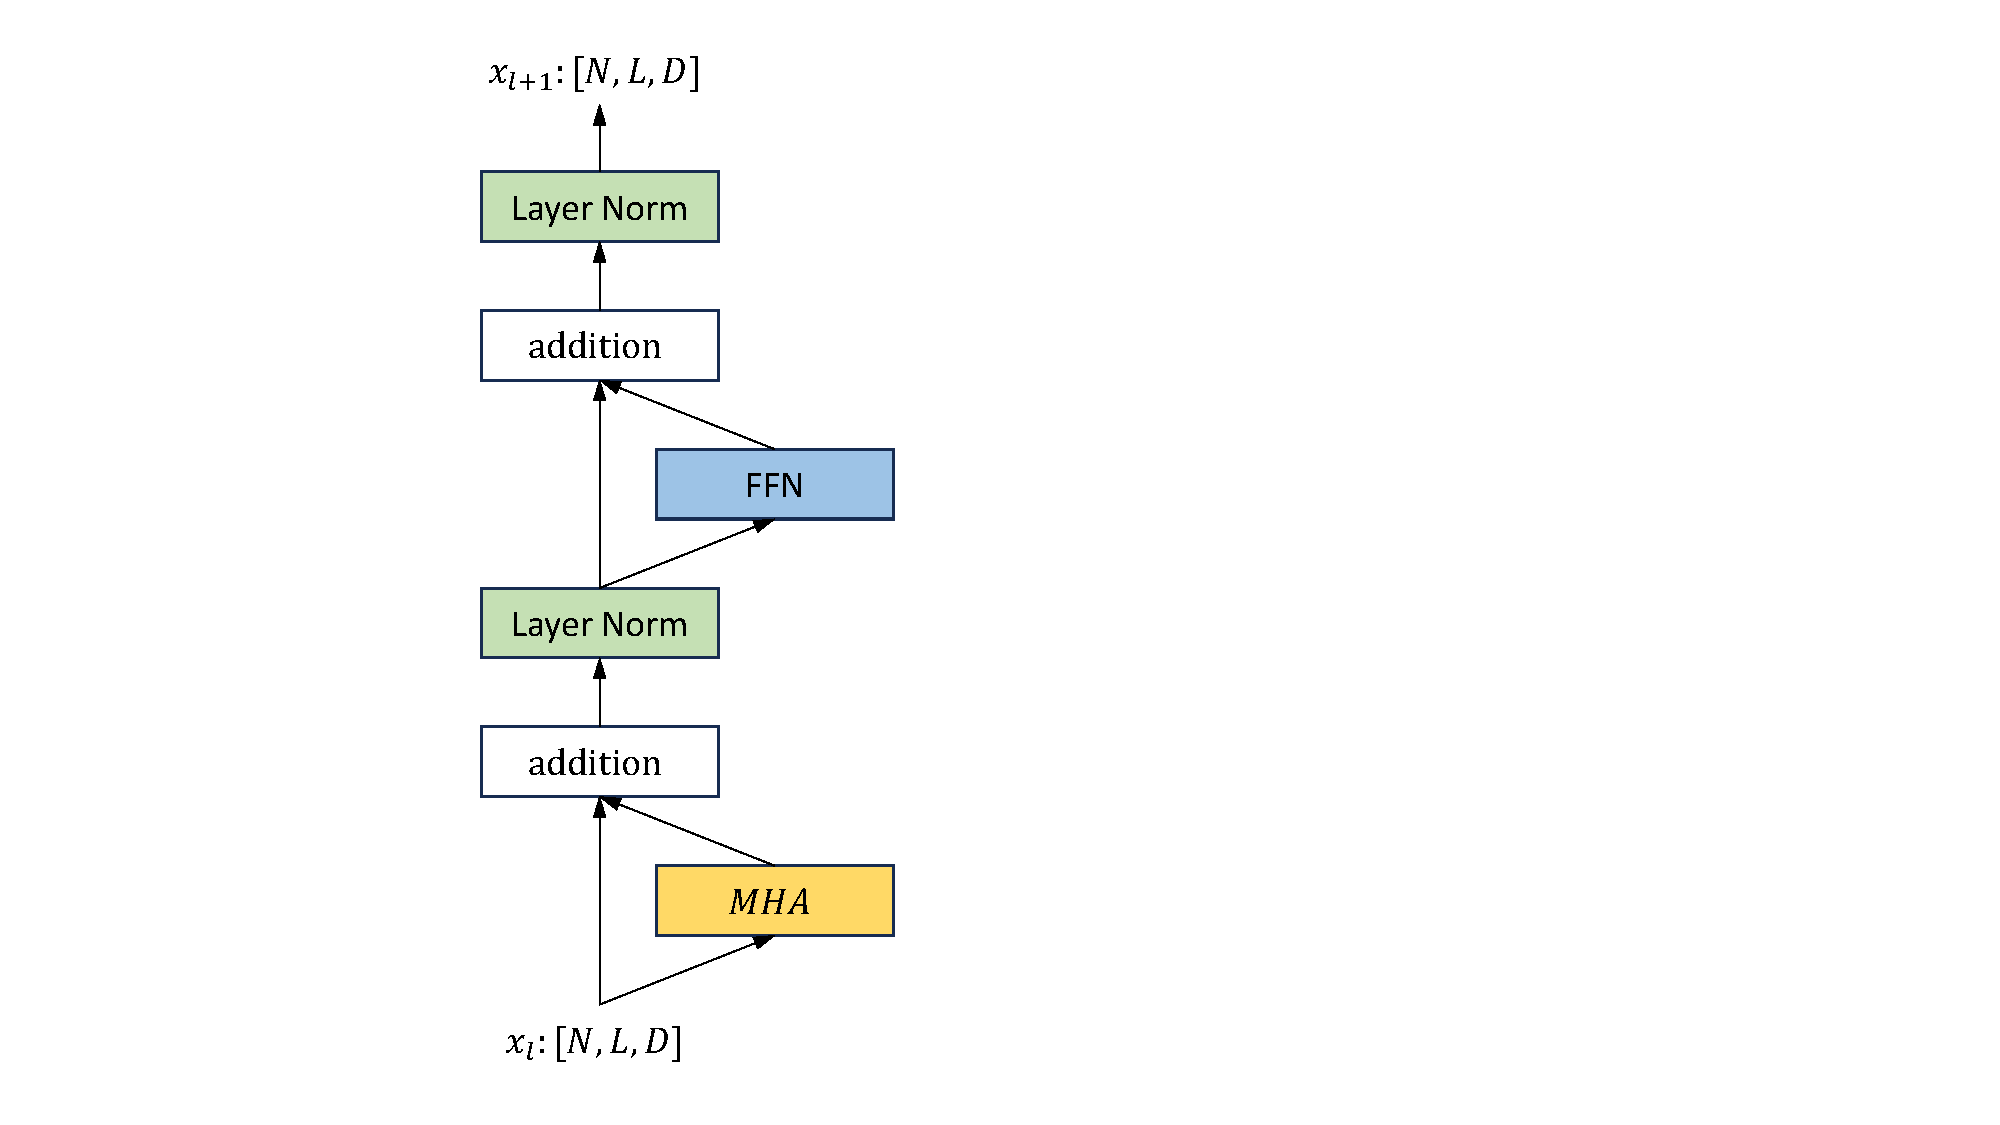
\includegraphics[width=3cm]{figures/Transformer-block.pdf}
    }
    \subfigure[Fused transformer block]{
    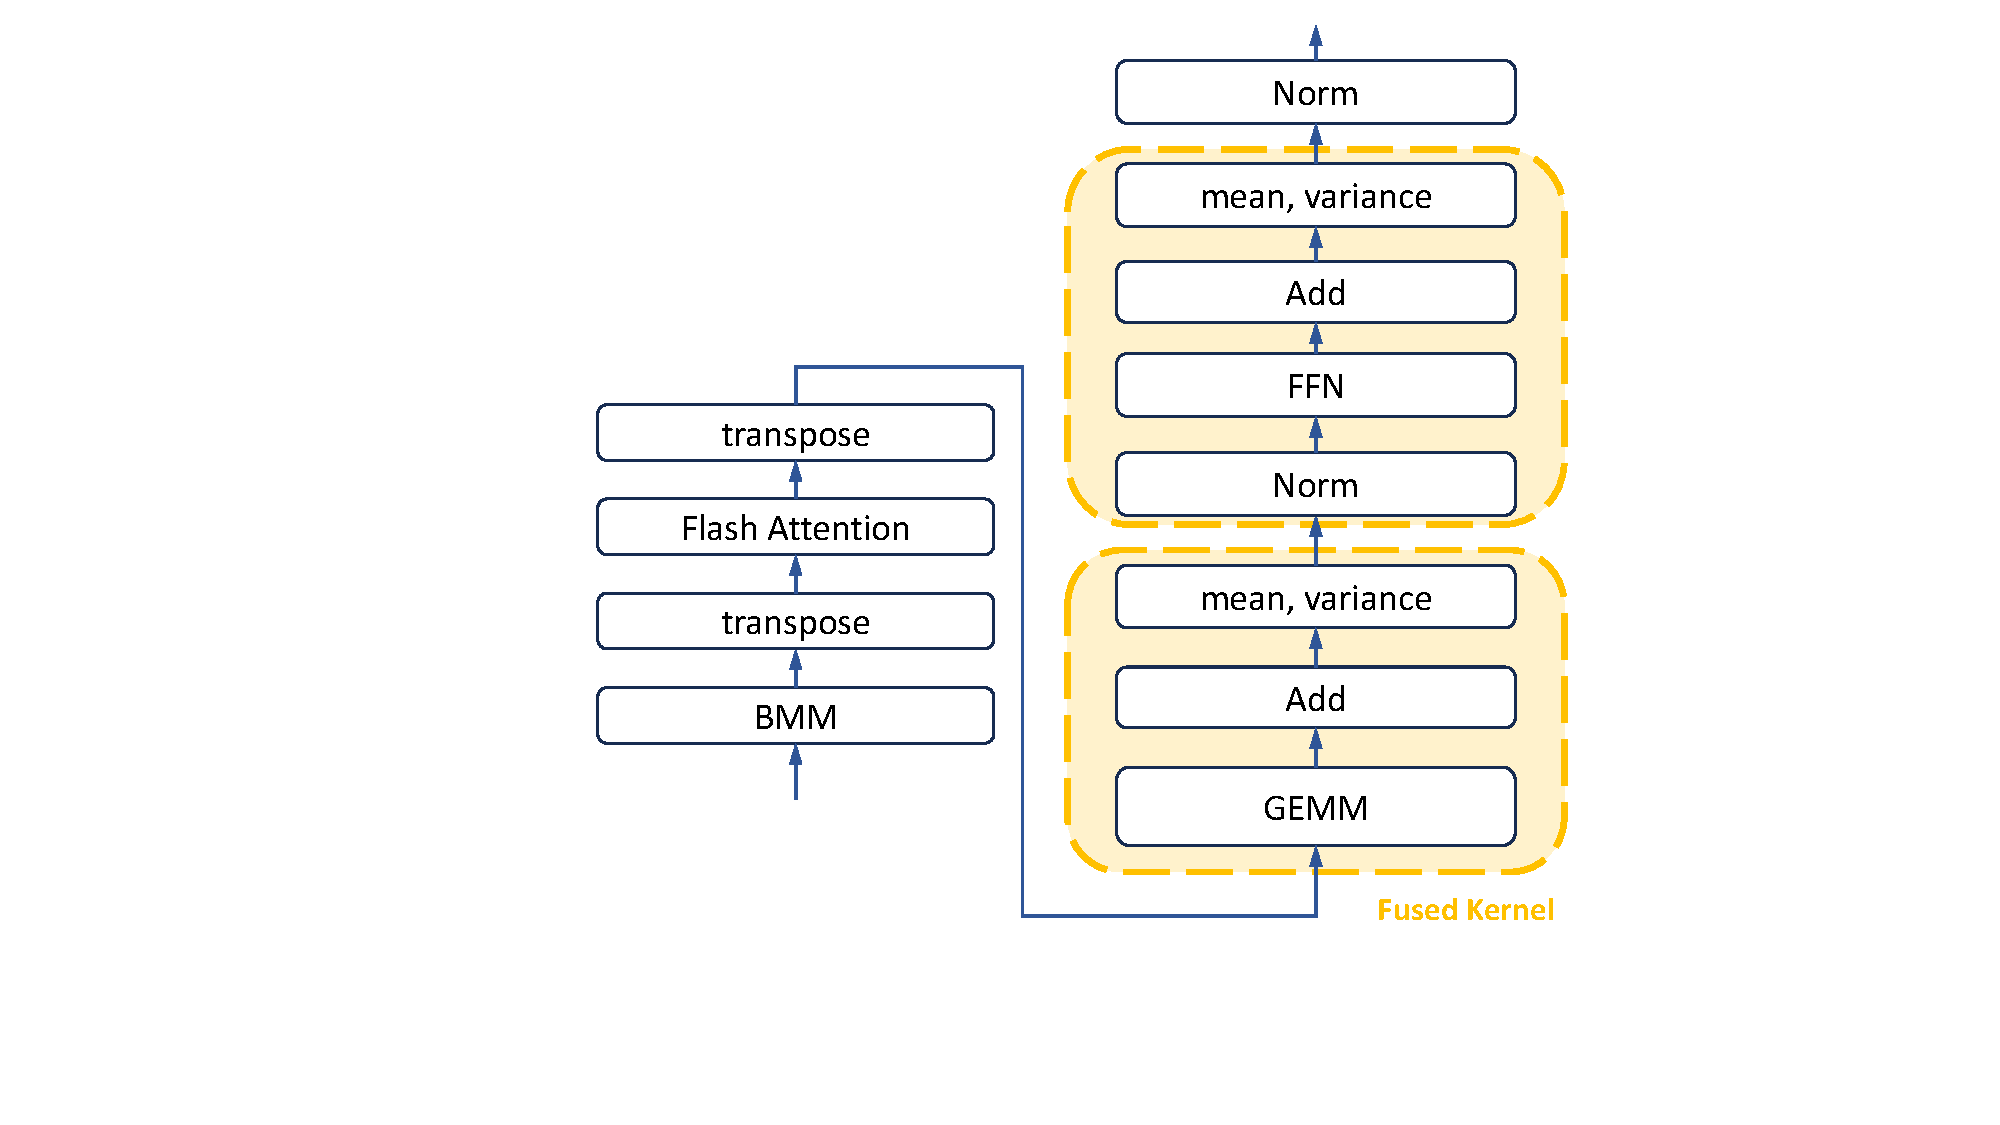
\includegraphics[width=7.5cm]{figures/fused_transformer_block.pdf}
    }
    \caption{Transformer block and a possible fusion plan.}\label{transformer-block}
\end{figure}
\vspace{-0.1cm}

The transformer model consists of a series of transformer blocks that are stacked on top of each other.
A transformer block is as shown above.

\subsection{MHA}

% \begin{align*}
% Q&=xW_q + b_q\\
% K&=xW_k + b_k\\
% V&=xW_v + b_v \\
% Q&=\text{transpose}(Q) \\
% K&=\text{transpose}(K) \\
% V&=\text{transpose}(V) \\
% O&=\text{softmax}(QK^T)V \\
% O&= \text{transpose}(O) \\
% O&=O W_o + b
% \end{align*}

\begin{figure}[h]
    \centering
    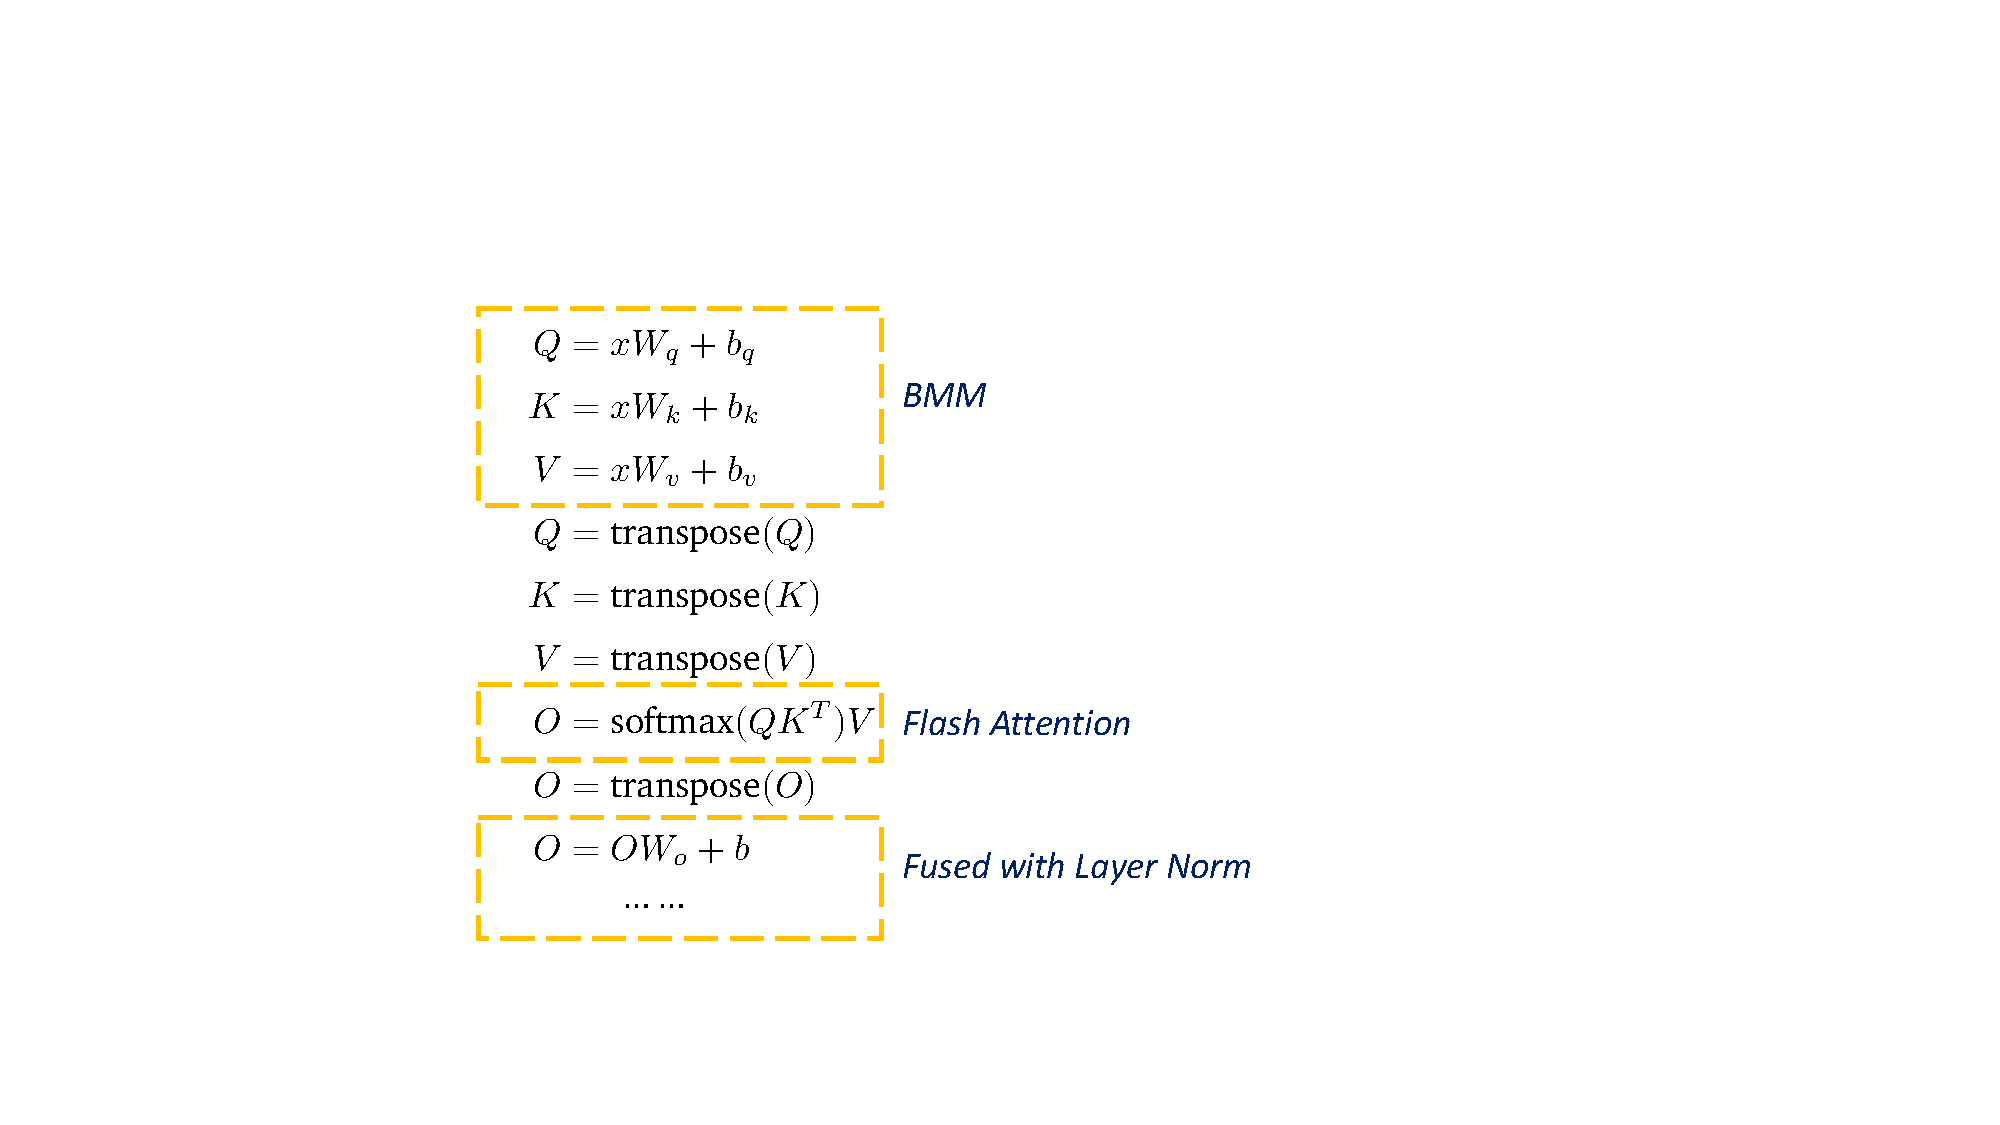
\includegraphics[width=0.4\textwidth]{figures/fused_mha.pdf}
    \caption{The fusion plan for MHA.}
\end{figure}

% \begin{table}[!htbp]
%     % \footnotesize
%     \setlength{\tabcolsep}{4pt}
%     \centering
%     \caption{Input tensors and their shapes.}
%     \begin{tabular}{c|l}
%     \textbf{Input}&\textbf{Shape} \\\midrule
%     $x \times W_Q$&$[N \times L, D] \times [D, D]$ \\
%     $x \times W_K$&$[N \times L, D] \times [D, D]$ \\
%     $x \times W_V$&$[N \times L, D] \times [D, D]$ \\
%     \end{tabular}
% \end{table}

\subsection{Layer Normalization}

$$y = \text{layernorm}(oW_o + b + x)$$

Input tensor $x$ has a shape of $N \times L \times D$ where $N$ stands for batch size, $L$ stands for sequence length, and $D$ stands for hidden size.
In the original Transformer, $D = 512$.

$$y_i=\frac{x_i-\mu}{\sqrt{\sigma^2 + \epsilon}}*\gamma_i+\beta_i\ \ \ i = [0, \ldots D-1]$$

Be definition:
\begin{align*}
    \mu_N &= \frac{1}{N}\sum_{i=1}^{N}x_i \\
    \sigma_{N}^2&=\frac{1}{N-1}\sum_{i=1}^{N}(x_i-\mu_{N})^2 \\
\end{align*}

To compute layer noramlization blockwise, we must use welford's online algorithm\cite{welford1962note} to compute the variance $\sigma^2$.
Define a quantity called $s_N = \sum^{N}_{i=1}(x_i - \mu_{N})^2$:

$$s_{N}=s_{N-1}+(x_N-\mu_{N-1})(x_N-\mu_N)$$

\subsection{FFN}

$W_1$ has a shape of $D \times 4D$ and $W_2$ has a shape of $4D * D$.

$$\text{FFN}(x) =\max(0, xW_1+b_1)W_2+b_2$$

\begin{align*}
\end{align*}

\subsection{Multi-scale Attention}

\begin{align*}
v_1 &= QK^T * \text{mask}\\
v_2 &= |v_1|.\text{sum}(\text{dim}=-1).\text{clamp}(\text{min}=1) \\
O &= \frac{v_1}{v_2}V  \\
\end{align*}

\begin{table}[!htbp]
    % \footnotesize
    \setlength{\tabcolsep}{4pt}
    \centering
    \caption{Input tensors and their shapes.}
    \begin{tabular}{c|c}
    \textbf{Input}&\textbf{Shape} \\\midrule
    $Q$ & $[N, H, L, E]$ \\
    $K$ & $[N, H, E, L]$ \\
    $V$ & $[N, H, L, E]$ \\
    $M$(mask) & $[H, L, L]$
    \end{tabular}
\end{table}

$N$ stands for batch size, $H$ stands for head number, $L$ stands for sequence length and $E$ stands for head dimensionality.

% \begin{lstlisting}[language=code_example, caption={}]
% for (:$i_1 \leftarrow [0, N-1)$:)  // batch size
%     for (:$i_2 \leftarrow [0, H-1)$:)  // number heads
%         for (:$i_3 \leftarrow [0, L-1)$:)  // sequence length
%             for (:$i_4 \leftarrow [0, L-1)$:)  // sequence length
%                 (:$v_1[i_4]=\text{\textbf{\textcolor{tomato}{dot}}}(Q[i_1, i_2, i_3],K[i_1, i_2, i_4])\textbf{\textcolor{tomato}{*}}\  M[i_2, i_3, i_4]$:)
%             (:$v_2 = $:)reduce(:($\textbf{\textcolor{tomato}{+}}, 0, \text{\textbf{\textcolor{tomato}{abs}}}(v_1))$:)
%             (:$O[i_1, i_2, i_3]=v_1V[i_1, i_2, i_3] \ \textbf{\textcolor{tomato}{/}}\ \textcolor{tomato}{\textbf{max}}(v_2, 1.)$:)  // [1, head_dim] x [head_dim, 1]
% \end{lstlisting}

\begin{figure}[h]
    \centering
    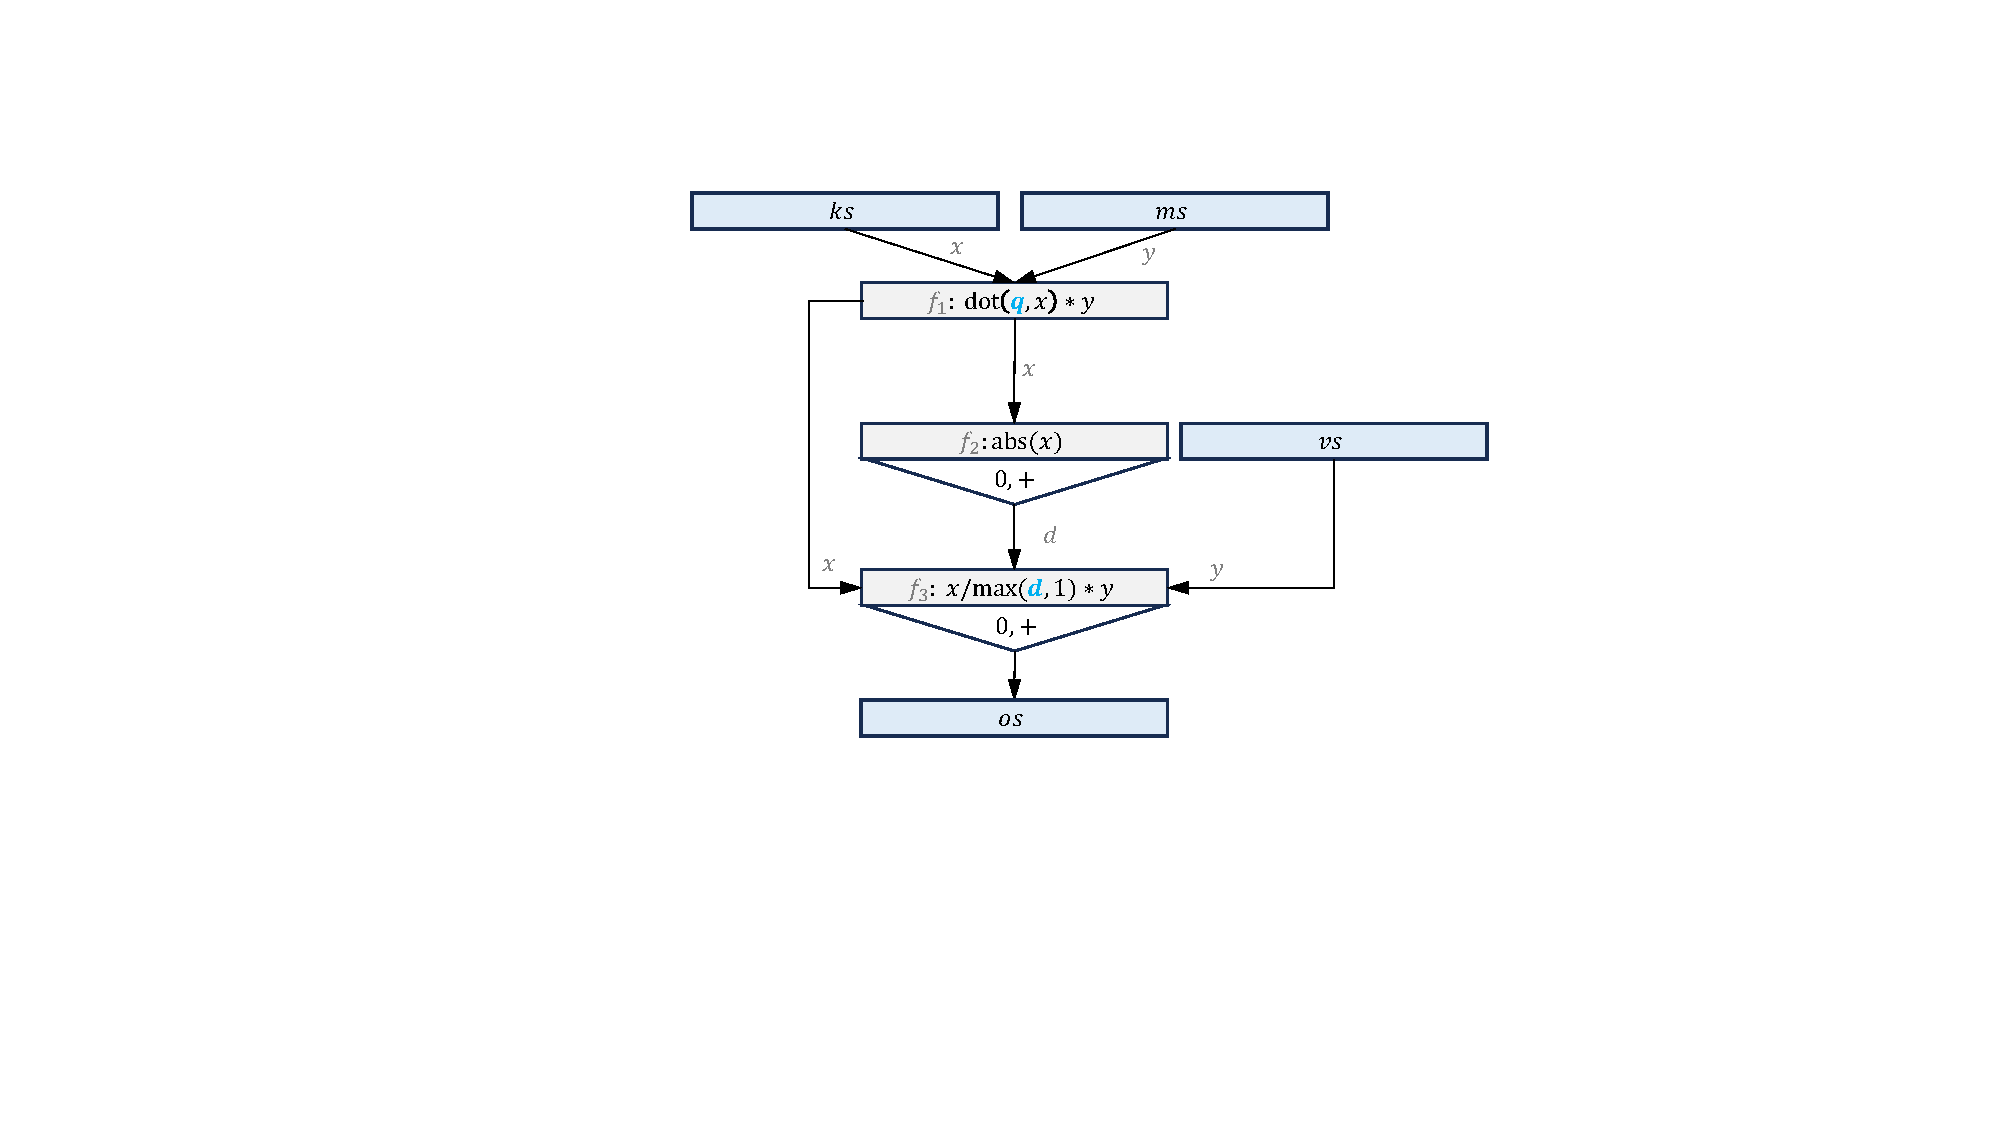
\includegraphics[width=0.65\textwidth]{figures/multi-scale-attn1.pdf}
    \caption{The multi-scale attention: the original computional flow.}
\end{figure}

\begin{figure}[h]
    \centering
    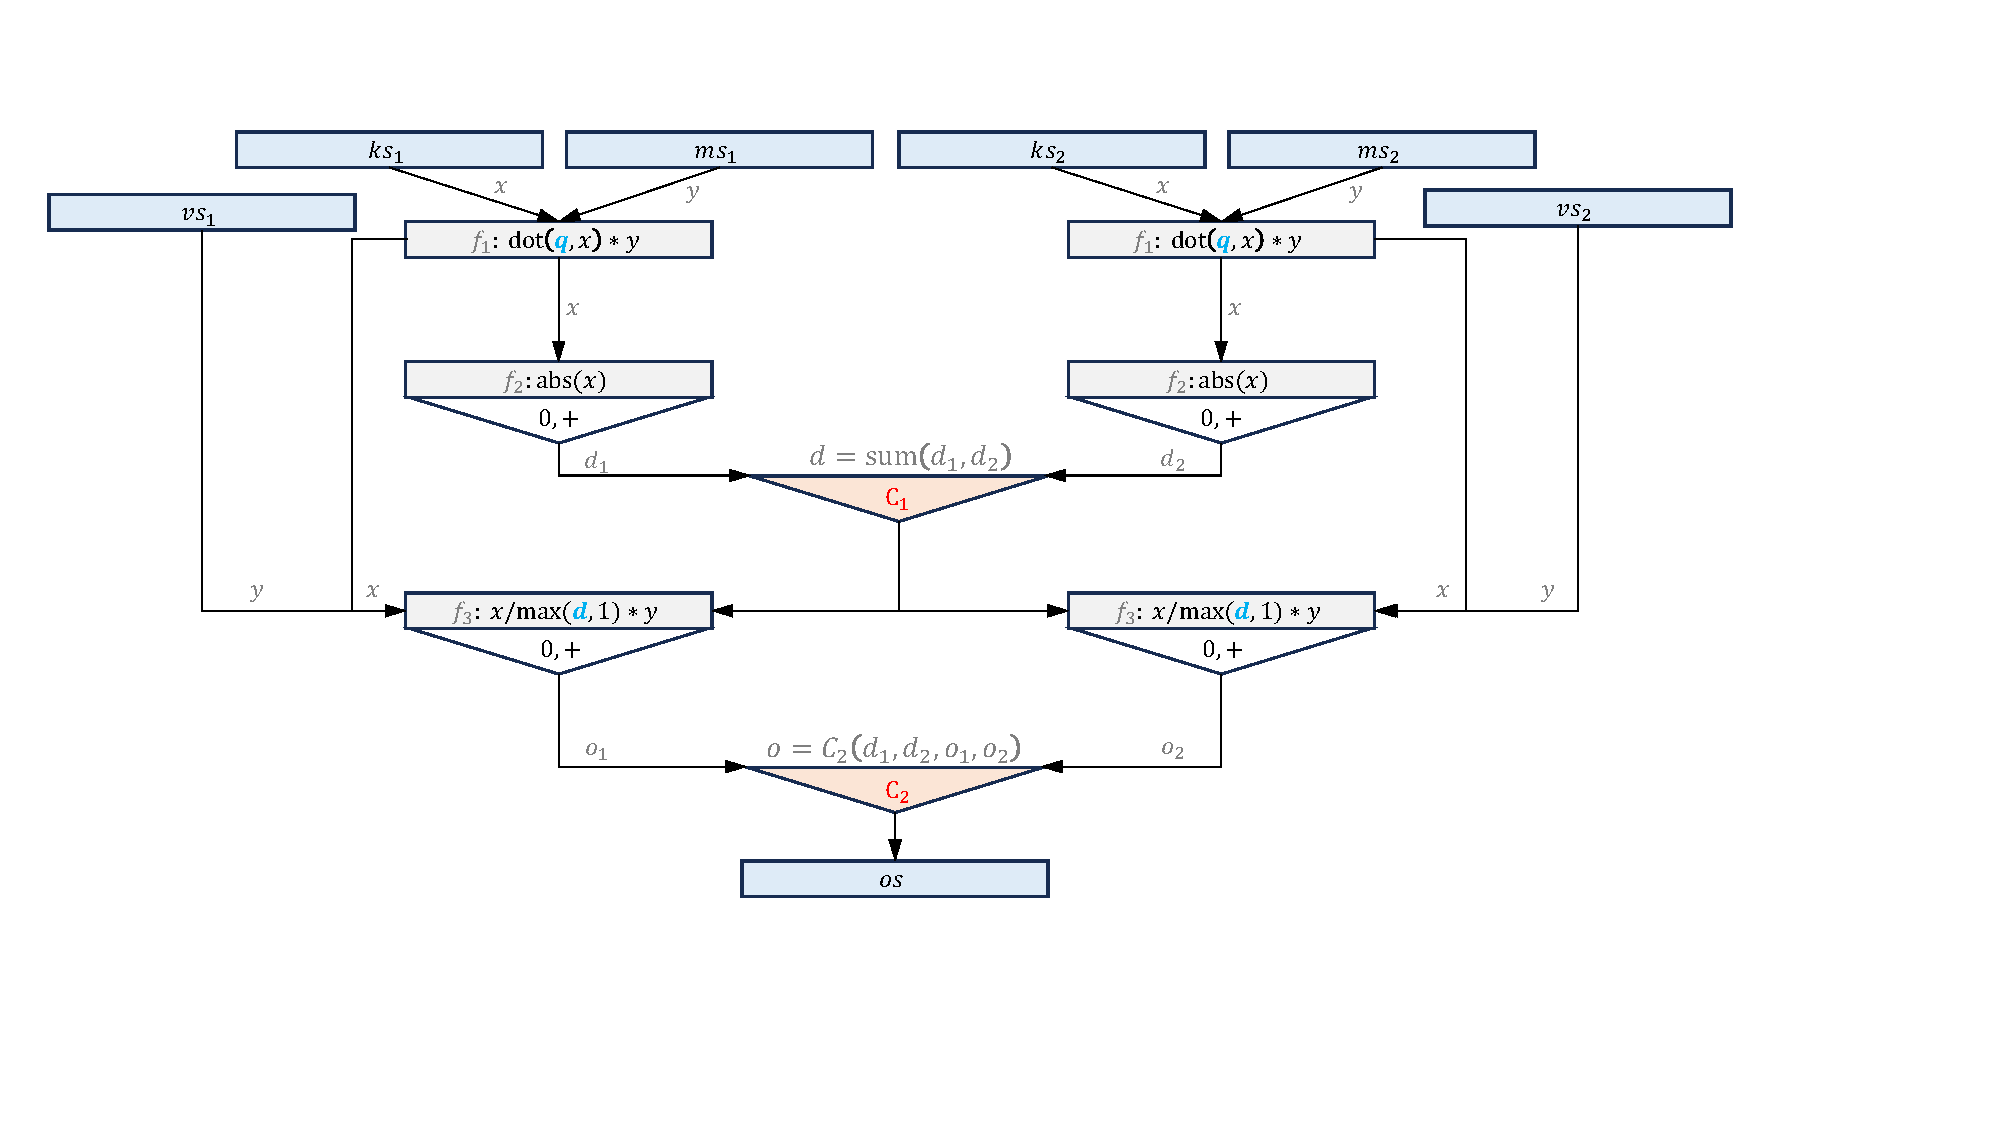
\includegraphics[width=1.\textwidth]{figures/multi-scale-attn2.pdf}
    \caption{The multi-scale attention: the expected computational flow.}
\end{figure}

$C_1$ is trivial:
$$C_1(d_1, d_2) = d_1+d_2$$

Consider $\bar{o}_1 = \frac{\bar{x}_1*\bar{y}_1}{d_1}$ has been computed for a single block, but a new constant $d'=\max(d_1, 1)$ has to be broadcast to the entire list $\bar{x}_1$ to compute a new output $\bar{o}_1'=\frac{\bar{x}_1*\bar{y}_1}{d_1'}$.

\begin{align*}
    \bar{x}_1*\bar{y}_1 &= d_1*\bar{o}_1 \\
    \bar{o}_1' &= \frac{\bar{x}_1*\bar{y}_1}{d'} = \frac{d_1 * \bar{o}_1}{d'}
\end{align*}

Similarly: $\bar{o}_2' = \frac{\bar{x}_2*\bar{y}_2}{d'} = \frac{d_2 * \bar{o}_2}{d'}$, therefore:

\begin{align*}
o&=\bar{o}_1'+\bar{o}_2' \\
&=\frac{1}{d'}(d_1*\bar{o}_1+d_2\bar{o}_2)
\end{align*}

\begin{align*}
\bar{v} &= [\bar{v}_1:\bar{v}_2] \\
r_1 &= \text{sum}(\bar{v}_1) & r_2 &= \text{sum}(\bar{v}_2) \\
d_1 &=\max(r_1, 1) &d_2 &= \max(r_2, 1) \\
\end{align*}

$\max(\text{sum}(r_1, r_2), 1) \ne \max(\text{sum}(\bar{v}), 1)$.

\textbf{Inputs}: $r_{i-1}:[B_r, 1]$,$d_{i-1}:[B_r,1]$, $o_{i}:[B_r, d]$, $q_i: [B_r, d]$, $k_i: [d, B_c]$, $v_i : [d, B_c]$, $m_i : [B_r, B_c]$

\textbf{Outputs}: $r_i:[B_r, 1]$, $d_{i}:[B_r, 1]$, $o_{i}:[B_r,d]$

\begin{lstlisting}[language=code_example, caption={Fused multi-scale attention kernel.}]
// o and d are accumulators
// q, k, v, m are input tiles
for (:$\textcolor{tomato}{r_{i-1}}, \textcolor{tomato}{d_{i-1}}, \textcolor{tomato}{o_{i-1}}, q_i, k_i, v_i, m_i \leftarrow i = [0, \frac{L}{B_c})$:) 
  // compute partial results for the current tile
  (:$t_i = q_i@k_i*m_i$:)
  (:$\bar{r}_i = \text{sum}(\text{abs}(t_i), \text{dim=-1}))$:)
  (:$o_{prev} = t_i@v_i$:)
  
  // update accumulators 
  (:$\bar{o}_i = d_{i-1} * o_{i-1} + o_{prev}$:)
  (:$\textcolor{tomato}{r_i} = r_{i-1} + \bar{r}_i$:)
  (:$\textcolor{tomato}{d_i} = \max(r_i, \mathbf{1}.)$:)
  (:$\textcolor{tomato}{o_i} = \bar{o}_i/d_i$:)
\end{lstlisting}
\clearpage
\begin{appendices}
\section{Welford Algorithm for Calculating Variance}

We want to calculate the mean and unbiased variance of a numeric list $X=[x_1 \ldots x_{N}]$ that has a length $N$:

\begin{align*}
\mu_{N} &= \frac{1}{N}\sum^{N}_{i=1} x_i \\
\sigma^2_{N} &=\frac{1}{N-1} \sum^{N}_{i-1}\left(x_i - \mu_{N}\right)^2 
\end{align*}

The two computations mentioned above scan the input list elements twice, each with a complexity of $O(N)$. Now, suppose we add a new element $x_{N}$ to the list and want to update the mean $\mu_{N+1}$ and variance $\sigma_{N+1}$. Instead of repeating the two $O(N)$ computations, can we update $\mu_{N+1}$ and $\sigma_{N+1}^2$ using the existing values of $N$, $\mu_{N}$, and $\sigma_{N}^2$? If so, we can compute $\mu_N$ and $\sigma_{N}^2$ for the entire list portion by portion for extremely long lists.

Let's start from the new mean $\mu_{N+1}$ from $x_{N+1}$ and $\mu_{N}$. This is rather straightforward:

\begin{align}
\mu_{N+1} &= \frac{x_{N+1}+N\mu_{N}}{N+1} \nonumber \\
&=\mu_{N}+\frac{x_{N+1}-\mu_{N}}{N+1}\tag{1}\label{eq:1}
\end{align}

Subsitute $N+1$ with $N$ in equation \eqref{eq:1}, we can also get:

\begin{equation}
\mu_{N}=\mu_{N-1}+\frac{x_{N}-\mu_{N-1}}{N}\tag{2}\label{eq:2}
\end{equation}


Let's define a quantity called $s_N$:

\begin{align*}
s_{N} &= \sum^{N}_{i=1}(x_i - \mu_{N})^2 \\
&=\sum^{N-1}_{i=1}\left(x_i-\mu_{N}\right)^2+\left(x_N-\mu_{N}\right)^2 \tag{3}\label{eq:3}
\end{align*}

Substitue equation \eqref{eq:2} into equation \eqref{eq:3}:

\begin{align*}
s_N &= \sum_{i=1}^{N-1}\left(x_i-\mu_{N-1}-\frac{x_N-\mu_{N-1}}{N} \right)^2 + \left(x_N-\mu_{N-1}-\frac{x_N-\mu_{N-1}}{N}\right)^2 \\
&=\sum_{i=1}^{N-1}\left(\left(x_i-\mu_{N-1}\right)-\frac{1}{N}\left(x_N-\mu_{N-1}\right)\right)^2+\left(\frac{N-1}{N}(x_N-\mu_{N-1})\right)^2 \tag{4}\label{eq:4}
\end{align*}

Let's first look into the first component of equation \eqref{eq:4}:

\begin{align*}
&\sum_{i=1}^{N-1}\left(\left(x_i-\mu_{N-1}\right)-\frac{1}{N}\left(x_N-\mu_{N-1}\right)\right)^2 \\
=&\sum_{i=1}^{N-1}\left((x_i-\mu_{N-1})^2-\textcolor{red}{\frac{2}{N}(x_i-\mu_{N-1})(x_N-\mu_{N-1})}+(x_N-\mu_{N-1})^2\right) 
\end{align*}

The equation in red is actually equal to zero.

\begin{align*}
&\sum_{i=1}^{N-1}\frac{2}{N}(x_i-\mu_{N-1})(x_N-\mu_{N-1}) \\
=&\frac{2}{N}(N-1)(x_N-\mu_{N-1})\left(\sum_{i=0}^{N-1}x_i-(N-1)\mu_{N-1}\right) \\
=&\frac{2}{N}(N-1)(x_N-\mu_{N-1})\left(\sum_{i=0}^{N-1}x_i-\sum_{i=0}^{N-1}x_i\right) \\
=&\ 0
\end{align*}

Substitue these results into equation \eqref{eq:4}:

\begin{align*}
s_{N} &=\sum_{i=1}^{N-1}\left((x_i-\mu_{N-1})^2+\frac{1}{N}(x_N-\mu_{N-1})^2\right) + \left(\frac{N-1}{N}(x_N-\mu_{N-1})\right)^2 \\
&=\frac{N-1}{N^2}(x_N-\mu_{N-1})^2+\frac{(N-1)^2}{N^2}(x_N-\mu_{N-1})^2+\sum_{i=1}^{N-1}(x_i-\mu_{N-1})^2 \\
&=\left[\frac{N-1}{N^2} + \frac{(N-1)^2}{N^2}\right](x_N-\mu_{N-1})^2+\sum_{i=1}^{N-1}\left(x_i-\mu_{N-1}^2\right) \\
s_N&=s_{N-1} + \frac{N-1}{N}(x_N-\mu_{N-1})^2 \tag{5}\label{eq:5}
\end{align*}

We can manipulate equation \eqref{eq:5} further by given:
\begin{align*}
(N-1)\mu_{N-1} &= N\mu_N-x_N \\
\mu_{N-1} &= \frac{N\mu_{N}-x_N}{N-1}
\end{align*}

substitute it into equation \eqref{eq:5}:

\begin{align*}
s_N&=s_{N-1} + (x_N-\mu_{N-1})\frac{N-1}{N}(x_N-\frac{N\mu_{N}-x_N}{N-1}) \\
s_N&=s_{N-1} + (x_N-\mu_{N-1})(x_N-\mu_{N})
\end{align*}

Suppose we use Welford's algorithm to calculate the mean and variance for lists $A$ and $B$.
Now we want to obtain the mean and variance for $AB$, which is the concatenation of $A$ and $B$. To do this, we can use the formula described in \cite{chan1982updating}.

\begin{align*}
N_{AB} &= N_{A} + N_{B} \\
\delta &= \mu_B - \mu_A \\
\mu_{AB} &= \mu_A+\delta\frac{N_B}{N_{AB}} \\
M_{2, AB} &=M_{2,A}+M_{2,B}+\delta^2*\frac{N_A N_B}{N_{AB}}
\end{align*}
\section{Gradient Computation}

Let $\circ$ stands for elementwise multiplication.

\subsection{Flash Attention}

The standard attention:
$$\mathbf{S}=\mathbf{Q}\mathbf{K}^T \in \mathbb{R}^{N\times N},\quad \mathbf{P} = \text{softmax}(\mathbf{S}) \in \mathbb{R}^{N \times N},\quad \mathbf{O} = \mathbf{PV}\in \mathbb{R}^{N\times d}$$

% Given $\mathbf{O}$, $\mathbf{Q}$, $\mathbf{K}$, $\mathbf{V}$, $\mathbf{dO}$ the backward pass propagates gradient $\mathbf{dO}$ from the output to the inputs.
% Let's compute back propagation $\mathbf{dQ}$, $\mathbf{dK}$ and $\mathbf{dQ}$ by hands.

If we have the matrices $\mathbf{O}$, $\mathbf{Q}$, $\mathbf{K}$, $\mathbf{V}$, and $\mathbf{dO}$, the backward pass propagates the gradient $\mathbf{dO}$ from the output to the inputs.
To compute the back propagation of $\mathbf{dQ}$, $\mathbf{dK}$, and $\mathbf{dV}$ by hand, we can follow the steps of the backpropagation algorithm.
Let's first consider a scalar loss function $\phi$ and an output gradient $\mathbf{dO}$ with dimensions $\mathbb{R}^{N\times d}$.

To obtain the gradient of $\mathbf{V}$ in matrix notation, we can simply use the following formula: $\mathbf{dV} = \mathbf{P}^T\mathbf{dO}$. This means that the blockified version can be expressed as follows:

\begin{equation}
\mathbf{dV}_j = \sum_i \mathbf{P}_{ij}^T\mathbf{dO}_i = \sum_{i}\frac{\exp({\mathbf{K}_j}^T\mathbf{Q}_i)}{\mathbf{L}_i}\mathbf{dO}_i \label{eq:mha1}
\end{equation}

We can then move on to computing $\mathbf{dP}$ using the formula $\mathbf{dP} = \mathbf{dOV}^T$. In blockified form, this can be expressed as follows: 
$$\mathbf{dP}_{ij}=\mathbf{dO}_i\mathbf{V}_j^T$$

Since the Jacobian of $\bar{y} = \text{softmax}(\bar{x})$ is represented by the matrix $\mathbf{J}_{\bar{x}}=\text{diag}(\bar{y})-\bar{y}^T\bar{y}$ where $\bar{x}$ and $\bar{y}$ are row vectors, we can use this to derive the following:

$$\mathbf{dS}_{i:}=(\text{diag}(\mathbf{P}_{i:})-\mathbf{P}^T_{i:}\mathbf{P}_{i:})\mathbf{dP}_{i:}=\mathbf{P}_{i:}\circ \mathbf{dP}_{i:}-\mathbf{P}_{i:}\textcolor{red}{(\mathbf{P}_{i:}^T \mathbf{dP}_{i:})}$$

Define: $$\mathbf{D}_i=\mathbf{P}_{i:}^T\mathbf{dP}_{i:}=\sum_j\frac{\exp({\mathbf{K}_j\mathbf{Q}_i^T})}{\mathbf{L}_i}\mathbf{dO}_i \mathbf{V}_j^T=\mathbf{dO}_i^T\sum_j\frac{\exp({\mathbf{Q}_i^T}\mathbf{K}_j)}{\mathbf{L}_i}\mathbf{V}_j = \mathbf{dO}_i^T\mathbf{O}_i$$

Then:
$$\mathbf{dS}_{i:}=\mathbf{P}_{i:}\circ\mathbf{dP}_{i:}-\mathbf{P}_{i:}\mathbf{D}_i$$

Hence:

$$\mathbf{dS}_{ij}=\mathbf{P}_{ij}\circ\mathbf{dP}_{ij}-\mathbf{P}_{ij}\mathbf{D}_i=\mathbf{P}_{ij}(\mathbf{dP}_{ij}-\mathbf{D}_i)$$

We can obtain $\mathbf{dQ}$ and $\mathbf{dK}$ in a blockified style by utilizing $\mathbf{dS}_{ij}$ and the following relationships: $\mathbf{dQ}=\mathbf{dS}\mathbf{K}$ and $\mathbf{dK}=\mathbf{dS}^T\mathbf{Q}$:

\begin{align}
\mathbf{dQ}_i &= \sum_{j}\mathbf{dS}_{ij}\mathbf{K}_j \notag\\
&= \sum_{j}\mathbf{P}_{ij}(\mathbf{dP}_{ij}-\mathbf{D}_i)\mathbf{K}_j \notag\\
&=\sum_j\frac{\exp(\mathbf{Q}_i^T\mathbf{K}_j)}{\mathbf{L}_i}(\mathbf{dO}_i\mathbf{V}_j^T-\mathbf{D}_i)\mathbf{K}_j \label{eq:mha2}\\
\mathbf{dK}_j &= \sum_i\mathbf{dS}_{ij}^T\mathbf{Q}_i \notag\\
&= \sum_i(\mathbf{dP}_{ij}^T-\mathbf{D}_i^T)\mathbf{P}_{ij}^T\mathbf{Q}_i \notag\\
&= \sum_i (\mathbf{V}_{j}\mathbf{dO}_i^T -\mathbf{D}_i^T)\frac{\exp(\mathbf{K}_j\mathbf{Q}_i^T)}{\mathbf{L}_i}\mathbf{Q}_i \label{eq:mha3}
\end{align}

Equations \eqref{eq:mha1}, \eqref{eq:mha2}, and \eqref{eq:mha3} describe a blockified computational process for obtaining $\mathbf{dQ}$, $\mathbf{dK}$, and $\mathbf{dV}$.

\subsection{Multi-scale Attention}

The multi-scale attention computes as:

$$\mathbf{S} = \mathbf{Q}\mathbf{K}^T\circ \mathbf{M} \in \mathbb{R}^{N\times N}, \quad \mathbf{P} = \frac{\mathbf{\bar{1}}}{\max(\text{rowsum}(\text{abs}(\mathbf{S})),\bar{\mathbf{1}})} \in \mathbb{R}^{N\times 1}, \quad \mathbf{O} = \mathbf{S}\mathbf{V} \circ \mathbf{P}\in \mathbb{R}^{N\times d}$$

To perform the backward computation, the system must compute the derivatives of $\mathbf{Q}$, $\mathbf{K}$,
and $\mathbf{V}$ with respect to the output $\mathbf{O}$, denoted as $\mathbf{dQ}$, $\mathbf{dK}$, and $\mathbf{dV}$, respectively.
The computation of $\mathbf{dV}$ in matrix notation is straightforward:
$$\mathbf{dV} = \mathbf{S}^T\mathbf{dO}\circ \mathbf{P}$$
And the blockified version of $\mathbf{\mathbf{dV}_j}$ is:

\begin{equation}
\mathbf{dV}_j = \sum_i \mathbf{S}_{ij}^T\mathbf{dO_i}\circ\mathbf{P}_i \label{eq:msa1}
\end{equation}

By applying the chain rule, the next step in the backward computation is to compute the derivative matrix $\mathbf{dP}$:

$$\mathbf{dP} = \text{rowsum}(\mathbf{dO} \circ \mathbf{SV})$$

The blockified version of $\mathbf{dP}_{ij}$ is:

$$\mathbf{dP}_{ij} = \text{sum}(\mathbf{dO}_i\circ\mathbf{S}_{ij}\mathbf{V}_j)$$

Computing $\mathbf{dS}$ is a somewhat a bit more complicated,
so it is best to break it down into smaller steps.
Let's assume the following to simplify the process:

\begin{align*}
\mathbf{y}_1 &= \text{abs}(\mathbf{S}) \\
\mathbf{y}_2 &= \text{rowsum}(\mathbf{y}_1) \\
\mathbf{y}_3 &= \max(\mathbf{y}_2, \mathbf{1}) \\
\mathbf{P} &= \frac{\mathbf{\bar{1}}}{\mathbf{y}_3}
\end{align*}

Then we can compute $\mathbf{dS}$ step by step:

\begin{align*}
    \frac{\mathbf{dP}}{\mathbf{dy}_3} & = -\frac{\mathbf{\bar{1}}}{\mathbf{y}_3 \circ \mathbf{y}_3}= -\mathbf{P}\circ \mathbf{P}\\
    \frac{\mathbf{dy}_3}{\mathbf{dy}_2} &\equiv \textcolor{red}{\nabla_{\max}}= \left\{
        \begin{aligned}
            &1, &\mathbf{y}_2 > \mathbf{\bar{1}}\\
            &0, &\mathbf{y}_2 \le \mathbf{\bar{1}}
        \end{aligned}
    \right. \\
    \frac{\mathbf{dy}_2}{\mathbf{dy}_1} &= \mathbf{\bar{1}}_{N\times N} \\
    \frac{\mathbf{dy}_1}{\mathbf{dS}} &\equiv \textcolor{red}{\nabla_{\text{abs}}}= \left\{
        \begin{aligned}
            &1, & \mathbf{S} \ge \mathbf{\bar{0}}\\
            &-1, & \mathbf{S} < \mathbf{\bar{0}}
        \end{aligned}
    \right.
\end{align*}

And:
\begin{align*}
    \frac{\mathbf{dP}}{\mathbf{dS}} &=\frac{\mathbf{dP}}{\mathbf{dy}_3}\circ \frac{\mathbf{dy}_3}{\mathbf{dy}_2} \circ \frac{\mathbf{dy}_2}{\mathbf{dy}_1} \circ \frac{\mathbf{dy}_1}{\mathbf{dS}} \\
    &= -\mathbf{P}\circ\mathbf{P} \circ \nabla_{\max} \circ \nabla_{\text{abs}}
\end{align*}

The blockified computation for $\frac{\mathbf{d\phi}_{ij}}{\mathbf{dS_{ij}}}=\mathbf{dS}_{ij}$ is:

\begin{align*}
\mathbf{dS}_{ij} &= - \text{sum}(\mathbf{dO}_i\circ \mathbf{S}_{ij}\mathbf{V}_i) \circ \mathbf{P}_{ij}\circ{\mathbf{P}_{ij}} \circ \textcolor{red}{\nabla_{\max}^{ij}} \circ \textcolor{red}{\nabla_{\text{abs}}^{ij}}\\
&=-\frac{\text{sum}(\mathbf{dO}_i\circ\mathbf{O}_i)}{\mathbf{P}_{ij}}\circ \mathbf{P}_{ij}\circ{\mathbf{P}_{ij}} \circ \textcolor{red}{\nabla_{\max}^{ij}} \circ \textcolor{red}{\nabla_{\text{abs}}^{ij}} \\
&=-\text{sum}(\mathbf{dO}_i\circ\mathbf{O}_i)\circ{\mathbf{P}_{ij}} \circ \textcolor{red}{\nabla_{\max}^{ij}} \circ \textcolor{red}{\nabla_{\text{abs}}^{ij}}
\end{align*}

where:

\begin{align*}
    \textcolor{red}{\nabla_{\max}^{ij}} &= \left\{
        \begin{aligned}
        &\mathbf{\bar{1}}, &\text{rowsum}(\text{abs}(\mathbf{S}_{ij})) \ge \mathbf{\bar{1}}\\
        &\mathbf{\bar{0}}, &\text{rowsum}(\text{abs}(\mathbf{S}_{ij})) < \mathbf{\bar{1}}\\
        \end{aligned}
    \right. \\
    \textcolor{red}{\nabla_{\text{abs}}^{ij}} &= \left\{
        \begin{aligned}
        &\mathbf{\bar{1}}, &\text{abs}(\mathbf{S}_{ij}) \ge \mathbf{\bar{0}}\\
        &\mathbf{-\bar{1}}, &\text{abs}(\mathbf{S}_{ij}) < \mathbf{\bar{0}}\\
        \end{aligned}
    \right.
\end{align*}

We can obtain $\mathbf{dQ}$ and $\mathbf{dK}$ in a blockified style by utilizing $\mathbf{dS}_{ij}$ and the following relationships: $\mathbf{dQ}=\mathbf{dS}\mathbf{K}\circ \mathbf{M}$ and $\mathbf{dK}=\mathbf{dS}^T\mathbf{Q}\circ \mathbf{M}$:

\begin{align}
\mathbf{dQ}_i &= \sum_j \mathbf{dS}_{ij}\mathbf{K}_j\circ \mathbf{M}_{ij} \notag\\
&= -\sum_{j}\text{sum}(\mathbf{dO}_i\circ\mathbf{O}_i)\circ{\mathbf{P}_{ij}} \circ \textcolor{red}{\nabla_{\max}^{ij}} \circ \textcolor{red}{\nabla_{\text{abs}}^{ij}}\mathbf{K}_j\circ \mathbf{M}_{ij}  \label{eq:msa2}\\
\mathbf{dK}_j &= \sum_i\mathbf{dS}_{ij}^T\mathbf{Q}_i\circ \mathbf{M}_{ij} \notag\\
&=-\sum_i\left(
    \text{sum}(\mathbf{dO}_i\circ\mathbf{O}_i)\circ{\mathbf{P}_{ij}} \circ \textcolor{red}{\nabla_{\max}^{ij}} \circ \textcolor{red}{\nabla_{\text{abs}}^{ij}}
    \right)^T \mathbf{Q}_i \circ \mathbf{M}_{ij} \label{eq:msa3}
\end{align}

Equations \eqref{eq:msa1}, \eqref{eq:msa2}, and \eqref{eq:msa3} describe a blockified computational process for obtaining $\mathbf{dQ}$, $\mathbf{dK}$, and $\mathbf{dV}$.


% Simplify equations above, we obtain:

% \begin{align}
% \mathbf{dS}&=\mathbf{dP} \circ \nabla_{\max}\circ \nabla_{\text{abs}} \notag\\
% &=-\frac{\text{rowsum}(\mathbf{O}\circ \mathbf{dO})}{\mathbf{P}}\circ \nabla_{\max} \circ \nabla_{\text{abs}}
% \end{align}


% Then we can compute $\mathbf{dQ}$ and $\mathbf{dK}$:

% \begin{align}
%     \mathbf{dQ} &= \mathbf{dS}\mathbf{K}^T\circ \mathbf{M} \notag \\
%     & = - \frac{\text{rowsum}(\mathbf{O}\circ \mathbf{dO})}{\mathbf{P}} \circ \nabla_{\max} \circ \nabla_{\text{abs}} \mathbf{K}^T\circ \mathbf{M} \label{eq:msa2} \\
%     \mathbf{dK} &= \mathbf{Q}^T\mathbf{dS}\circ \mathbf{M} \notag \\
%     &= -\mathbf{Q}^T \frac{\text{rowsum}(\mathbf{O}\circ \mathbf{dO})}{\mathbf{P}} \circ \nabla_{\max} \circ \nabla_{\text{abs}} \circ \mathbf{M}\label{eq:msa3}
% \end{align}

% represent the gradient computations for multi-scale attention. Now, let's consider how we can blockify the entire gradient computation process.

% \begin{align*}
% \mathbf{dV}_j &= \mathbf{K}_j\sum_{i}\frac{\mathbf{Q}_i^T\mathbf{dO}_i}{\mathbf{P}_{ij}} \\
% \mathbf{dK}_j &= -\sum_{i}\mathbf{Q}_i^T\frac{\text{rowsum}(\mathbf{O}_i^T\mathbf{dO}_i)}{\mathbf{P}_i}\circ \nabla_{\max}^i\circ \nabla_{\text{abs}}^{ij}\circ \mathbf{M}_{ij} \\
% \mathbf{dQ}_i &= -\frac{\text{rowsum}(\mathbf{O}_i \circ \mathbf{dO}_i)}{\mathbf{P}_i}\circ \nabla_{\max}^i\sum_j \nabla_{\text{abs}}^{ij}\circ \mathbf{M}_{ij}
% \end{align*}
\end{appendices}

\clearpage
\bibliographystyle{abbrv}
\bibliography{references.bib}

\end{document}